Finding the convex hull is a fundamental problem in computational geometry.
Quickhull is a fast algorithm for finding convex hulls.
In this paper, we present VQhull, a fast parallel implementation of Quickhull that exploits vector instructions and coordinates CPU cores in a way that minimizes data movement.
This implementation obtains a sequential runtime improvement of \qtyrange{1.6}{16}{\times}, and a parallel runtime improvement of \qtyrange{1.5}{11}{\times} compared to the state of the art on the Problem Based Benchmark Suite.
VQhull achieves \qtyrange{85}{100}{\percent} of the peak bandwidth on non\-/NUMA architectures, and \qtyrange{66}{78}{\percent} on a dual\-/CPU NUMA system.
This leaves little room for further improvements.

A \qty{4}{\times} speedup on 8 cores corresponds to a parallel efficiency of \qty{50}{\percent}.
This suggests a waste of energy, but our measurements show a more complicated picture: whereas in some cases parallelism improves energy efficiency, in other cases it significantly degrades it.
Quickhull serves as a case study showing that runtime and energy consumption do not necessarily go hand in hand, and that energy behaviour is highly platform and input dependent.

\section{Introduction}
The convex hull of a set of points is the smallest superset closed under taking convex combinations, a type of weighted average.
The convex hull of a finite set in 2D is a polygon, which can be described by its vertices.
Finding these vertices and listing them in order (clockwise or counterclockwise) is a fundamental algorithm in computational geometry.
Some problems make use of the convex hull construction directly, while others use a convex hull algorithm as a subroutine.
Applications can be found in a wide range of domains, such as collision detection~\cite{tang2008collision}, path planning~\cite{meeran1997optimum}, and urban planning~\cite{kang2017measuring}.

There exists a multitude of algorithms for finding the convex hull~\cite{graham1972efficient,jarvis1973identification,eddy1977convex,preparata1977convex,bykat1978convex,akl1978fast,andrew1979another,clarkson1993four,barber1996quick,chan1996optimal}.
The development of parallel algorithms started soon after the first convex hull algorithms were published~\cite{nath1981parallel}.
Though still theoretically interesting, these algorithms do not deliver on the goal of high performance on modern architectures.
More recent approaches~\cite{masnadi2020concurrent} rely on point filtering for most of the performance gain.
While valuable, this is orthogonal to convex hull algorithms on data that cannot be effectively filtered.
Relating runtime performance to peak performance of the hardware shows there is still significant room for improvement.
In this paper, we aim to close this gap by providing a novel parallelisation of the Quickhull algorithm called VQhull.

Moreover, the notion of performance is evolving.
Practical power limits already constrain real systems: data centres are increasingly bound by facility\-/level power delivery, and expansion or higher sustained load is often limited by what can be supplied to the building rather than by available compute hardware.
A concrete example is the Dutch \emph{Snellius} supercomputer, whose scale is constrained by a power budget.
In that setting, runtime alone is an incomplete objective.
Improving the energy efficiency of software directly increases how much useful work can be performed within a fixed power budget.
We therefore also describe a method for measuring energy consumption, and use it to evaluate the energy efficiency of our approach.

Our contributions are:
\begin{itemize}
  \item A vectorized algorithm for extracting two disjoint subsets in-place.
  (Section~\ref{sec:subset})
  \item An implementation of VQhull with a parallelized subset extraction over multiple cores in a bandwidth\-/friendly manner.
  (Section~\ref{sec:impl})
  \item An extensive runtime performance and energy consumption analysis of our approach compared to the state of the art, on three platforms.
  (Section~\ref{sec:evaluation})
\end{itemize}

\section{Background}

\subsection{Quickhull algorithm}
The Quickhull algorithm~\cite{barber1996quick} is a widely used technique for finding the convex hull of a finite point set.
It operates similarly to the QuickSort algorithm, as both apply a divide\-/and\-/conquer approach to recursively partition a set.
Figure~\ref{fig:quickhull} illustrates the basic idea behind Quickhull\---Algorithm~\ref{alg:quickhull}.
If we have three points $p$, $r$, $q$ on the convex hull of $P$, then the points inside that triangle are not in the convex hull and can be discarded.
The points $S_1$ to the left of $\overrightarrow{pr}$, and the points $S_2$ to the left of $\overrightarrow{rq}$ may be on the convex hull, and are recursively inspected.

To find three points on the convex hull, we can start with the leftmost and rightmost points $p$ and $q$.
We use the degenerate triangle $\Delta pqp$ to bootstrap the algorithm.
The arguments of the recursive function \code{Hull} give two points on the convex hulls of $S_1$, $S_2$.
To find the third point, we use the following observation.
If $x$, $y$ are on $CH(P)$, then a point $z \in P$ with maximum distance to $\overrightarrow{xy}$ must also be on the convex hull.

\begin{figure}[ht]
  \centering
  \begin{tikzpicture}
    \fill (0.0, 0.0) coordinate (p) circle (2pt);
    \fill (6.5, 0.8) coordinate (q) circle (2pt);
    \fill (2.3, 3.2) coordinate (r) circle (2pt);

    \node[anchor=north east] at (p) {$p$};
    \node[anchor=north west] at (q) {$q$};
    \node[anchor=south] at (r) {$r$};
    \node at (-0.25, 1.95) {$S_1$};
    \node at (5.15, 2.95) {$S_2$};

    \draw (p) -- (q);
    \draw[->,shorten >=2pt] (p) -- (r);
    \draw[->,shorten >=2pt] (r) -- (q);

    \foreach \x/\y in {
      0.55/1.25,
      0.90/2.35,
      1.80/1.00,
      2.65/1.95,
      3.75/2.70,
      4.30/1.55,
      5.80/2.35
    } {\fill (\x,\y) circle (2pt);}
  \end{tikzpicture}%
  \caption{An example of the first partitioning step of the Quickhull algorithm.}%
  \label{fig:quickhull}%
\end{figure}

\begin{algorithm}[ht]
  \begin{algorithmic}[1]
    \Require The set of points $P \subset \mathbb{R}^2$.
    \Ensure The vertices $H \subseteq P$ of the convex hull in clockwise order.
    \State Let $p \in P$ be the leftmost point.
    \State Let $q \in P$ be the rightmost point.
    \State $H := \{p\}$ $\cup$ \Call{Hull}{$P$, $p$, $q$, $p$}
    \Function{Hull}{$P$, $p$, $r$, $q$}
      \If{$|P| \leq 1$}
        \State \Return{$P$}
      \Else{}
        \State $S_1 := \{u \in P \mid u \text{ to the left of } \overrightarrow{pr}\}$
        \State $r_1 := \argmax\limits_{u \in S_1} d(u, \overrightarrow{pr})$
        \State $S_2 := \{u \in P \mid u \text{ to the left of } \overrightarrow{rq}\}$
        \State $r_2 := \argmax\limits_{u \in S_2} d(u, \overrightarrow{rq})$
        \State \Return{\Call{Hull}{$S_1$, $p$, $r_1$, $r$} $\cup$
                       $\{r\}$ $\cup$ \Call{Hull}{$S_2$, $r$, $r_2$, $q$}}
      \EndIf
    \EndFunction
  \end{algorithmic}%
  \captionof{algorithm}{Quickhull algorithm.}%
  \label{alg:quickhull}%
\end{algorithm}

We can efficiently and accurately tell whether $u$ is to the left of $\overrightarrow{pq}$ by testing
\[
(p_x - u_x) \cdot (q_y - u_y) > (p_y - u_y) \cdot (q_x - u_x)
\]
To find the farthest point in $S_1$ from $\overrightarrow{pr}$, we take a candidate point $u \in S_1$, iterate over the other points $u' \in S_1$, and then check whether $u$ is farther than $u'$ from $\overrightarrow{pq}$ by testing
\[
(r_y - p_y) (u_x - u'_x) < (r_x - p_x) (u_y - u'_y)
\]
(and similarly for the farthest point in $S_2$).

The partitioning step is then recursively applied in Algorithm~\ref{alg:quickhull} on the remaining subsets $S_1$ and $S_2$.
Each call adds the element of its subset with maximum distance to $\overrightarrow{xy}$ to the convex hull.

\subsection{Performance on CPUs}\label{sec:performance}
Implementation\-/related performance improvements come mainly from exposing parallelism and reducing data movement.
We review what this looks like on the hardware we target, a Central Processing Unit (CPU), so we can design the parallel algorithm with this in mind.

\paragraph{Branch prediction}
A CPU has multiple execution units per core.
If there are no dependencies between instructions, these units can execute instructions in parallel (\emph{instruction\-/level parallelism}), improving performance.
To keep a steady flow of instructions, the CPU will make a guess when encountering a conditional jump\---generated by if statements and loops in high\-/level languages.
This is called branch prediction and improves performance when guessed correctly.
If the guess is incorrect, the CPU must make an expensive recovery.
This trade-off is usually worthwhile because most branches are easy to predict, but Quickhull is an exception to this rule.

\paragraph{Vectorisation}
A \emph{vector} or \emph{SIMD} instruction is one that operates on multiple primitive types (such as integers or floating point numbers) at the same time.
The number of elements is called the \emph{vector width}, and is typically between $2$ and $8$ elements.

These instructions can be used to do multiple arithmetic operations such as \code{a[0] = b[0] + c[0]; a[1] = b[1] + c[1];} in one instruction, but also data movement such as \code{a[0] = flag[0] ? b[0] : c[0]; a[1] = flag[1] ? b[1] : c[1];}.
This reduces the number of instructions necessary, and instructions that permute data can also be used instead of branches.

\paragraph{Data movement and multithreading}
This parallelism increases the number of computations we can do in a given interval, but that is not the only limiting factor.
After all, we also need to load and store data fast enough.
We call applications limited by the number of computations we can do \emph{compute\-/bound}, and applications limited by data movement \emph{memory\-/bound}.
The main goal in optimizing memory\-/bound computations is to improve data locality, which shifts data movement from DRAM to caches.

Branch prediction and vectorisation happen on each core.
Similarly, each core also has some fast local memory called a cache.
These resources scale with using more cores.
Main memory, however, shares a common data bus with all cores.
For this reason, problems are more likely to become memory\-/bound when using more cores.

\section{Subset extraction}\label{sec:subset}
The main computation of Algorithm~\ref{alg:quickhull} is to extract subsets $S_1$, $S_2$ from $P$.
We first describe how to exploit SIMD parallelism for a single core, and then parallelize it over multiple cores.
Though the algorithm on one core is parallel in its use of SIMD instructions and out\-/of\-/order execution, we follow convention and call it sequential.

\subsection{Sequential extraction}
The main idea behind the extraction on a single CPU core is to classify multiple points simultaneously by using vector instructions.
These registers can hold multiple elements, and corresponding instructions can operate on all of them simultaneously.

The main instruction used is the compression instruction \code{vcompresspd}, from the Intel AVX-512 instruction set, illustrated in Figure~\ref{fig:compress}.
This instruction takes a vector register of \code{double}s and an integer whose bits encode which elements in the vector should be compressed.
It then stores these elements contiguously in memory.
We can emulate \code{vcompresspd} on CPUs with different instruction sets~\cite{wassenberg2022vectorized}.
The compression can be used to extract the subsets from a single vector register.
We can use this instruction twice to extract the elements of $S_1$ and $S_2$ from a vector register.

\begin{figure}[ht]
  \centering
  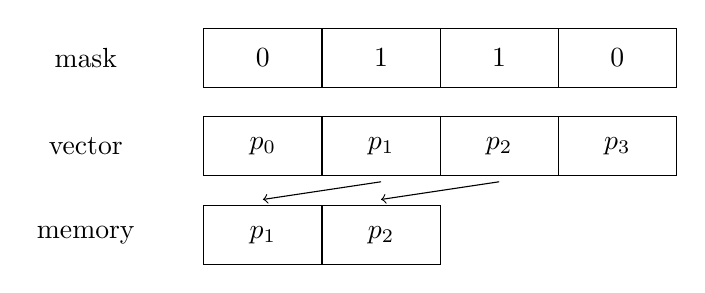
\begin{tikzpicture}[scale=1.5]
    \foreach \i in {0, ..., 3} {
      \draw (\i, 0) rectangle (\i + 1, 0.5) node[midway] {$p_{\i}$};
    }
    \draw (0, 0.75) rectangle (1, 1.25) node[midway] {$0$};
    \draw (1, 0.75) rectangle (2, 1.25) node[midway] {$1$};
    \draw (2, 0.75) rectangle (3, 1.25) node[midway] {$1$};
    \draw (3, 0.75) rectangle (4, 1.25) node[midway] {$0$};
    \draw (0, -0.75) rectangle (1, -0.25) node[midway] {$p_1$};
    \draw (1, -0.75) rectangle (2, -0.25) node[midway] {$p_2$};
    \draw [->] (1.5, -0.05) -- (0.5, -0.2);
    \draw [->] (2.5, -0.05) -- (1.5, -0.2);
    \node at (-1, 1) {\code{mask}};
    \node at (-1, 0.25) {\code{vector}};
    \node at (-1, -0.5) {\code{memory}};
  \end{tikzpicture}%
  \caption{The \code{vcompresspd} instruction.}%
  \label{fig:compress}%
\end{figure}

To extend the extraction to an entire array, we repeatedly use the compression instruction while maintaining an invariant illustrated in Figure~\ref{fig:invariant_qhull}.
Algorithm~\ref{alg:subset} maintains the following invariant, where $d$ is the number of elements per register:
\begin{enumerate}
  \item we have $P[0, w_l) \subseteq S_1$,
  \item we have $P[w_r, |P|) \subseteq S_2$,
  \item either $r_l - w_l \geq d$ or $w_r - r_r \geq d$,
  \item the unclassified points are in $P[r_l, r_r)$ or buffered.
\end{enumerate}

\begin{algorithm}[ht]
  \begin{algorithmic}[1]
    \Require A set of $n$ points $P \subset \mathbb{R}^2$.
    \Ensure Pointers $w_l$, $w_r$ and an in-place modification of $P$ such
    that $P[0, w_l) = S_1$ and $P[w_r, |P|) = S_2$.
    \State $w_l = 0$; $r_l = d$; $r_r = |P| - d$; $w_r = |P|$;
    \State bufL = $P[0, d)$; bufR = $P[n - d, n)$;
    \While{$r_l < r_r$}
      \If{$w_l - r_l \geq r_r - w_r$}
        \State reg = $P[r_l, r_l + d)$
        \State $r_l = r_l + d$
      \Else
        \State $r_r = r_r - d$
        \State reg = $P[r_r, r_r + d)$
      \EndIf
      \State extract $S_1$ from reg, write to $w_l$, increase $w_l$
      \State extract $S_2$ from reg, decrease $w_r$, write to $w_r$
    \EndWhile
    \State extract $S_1$, $S_2$ from bufL and bufR
  \end{algorithmic}%
  \captionof{algorithm}{Subset extraction.}%
  \label{alg:subset}%
\end{algorithm}

We establish the invariant with steps 1 and 2 of Algorithm~\ref{alg:subset}.
These buffered elements can be safely overwritten.
Our writes respect assertions 1 and 2.
We read $d$ elements from the side of the array where the distance between read and write pointer is smallest, ensuring that on that side no points are overwritten.
Assertion 3 ensures there are no points overwritten on the other side either, which implies 4.
Therefore, we only have to show that assertion 3 holds.
For this reason, we ensure at the initialisation of the algorithm that $(r_l - w_l) + (r_r - w_l) \geq 2d$.
As we read $d$ elements at each step, and write less than or equal to $d$ elements, this inequality is maintained.
The sum $(r_l - w_l) + (r_r - w_l)$ is at least $2d$, so the minimum $\min(r_l - w_l, r_r - w_l)$ is at least $d$.

\begin{figure}[ht]
  \resizebox{\linewidth}{!}{%
    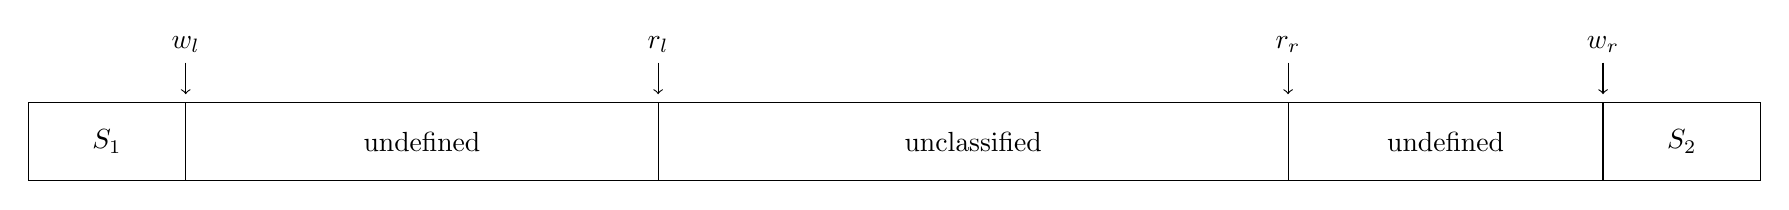
\begin{tikzpicture}
      \draw (0, 0)  rectangle (2, 1)  node[midway] {$S_1$};
      \draw (2, 0)  rectangle (8, 1)  node[midway] {\code{undefined}};
      \draw (8, 0)  rectangle (16, 1) node[midway] {unclassified};
      \draw (16, 0) rectangle (20, 1) node[midway] {\code{undefined}};
      \draw (20, 0) rectangle (22, 1) node[midway] {$S_2$};

      \draw[->] (2,  1.5) node[above] {$w_l$} -- (2,  1.1);
      \draw[->] (8,  1.5) node[above] {$r_l$} -- (8,  1.1);
      \draw[->] (16, 1.5) node[above] {$r_r$} -- (16, 1.1);
      \draw[->] (20, 1.5) node[above] {$w_r$} -- (20, 1.1);
    \end{tikzpicture}%
  }%
  \caption{Invariant for extracting the subsets $S_1$ and $S_2$ from a set of points $P$.}%
  \label{fig:invariant_qhull}%
\end{figure}

\subsection{Parallel extraction}
Extracting $S_1$ and $S_2$ has linear complexity, so it is very likely to be limited by bandwidth.
For this reason, minimizing data movement is the primary design goal of the parallel algorithm.
The algorithm consists of two conceptual steps.
First, we logically partition the points over the threads and have each thread independently extract subsets from their local part.
Second, we do a cleanup step that constructs the global subsets $S_1$, $S_2$ from the local parts.

\paragraph{Local extraction}
For the local extraction, we form a partition
\[
P = \bigcup\limits_{s = 0}^{t - 1} P^{(s)}
\]
over the $t$ total threads.
The most straightforward way would be to use a block distribution as in Figure~\ref{fig:block}.
We can then use the sequential extraction directly on each chunk.
However, this simplicity comes with a significant performance penalty when points are randomly ordered, which is a common scenario.
Each thread has points that need to be moved to the left or right side of the array.
However, the block partition gives each thread indices that are either on the left or the right side of the array.
This incurs significant data movement in the cleanup step, which we would like to avoid.

\begin{figure}[ht]
  \begin{subfigure}[b]{\linewidth}
    \resizebox{\linewidth}{!}{%
      \begin{tikzpicture}
        \draw (0, 0) rectangle (16, 0.5);
        \draw[fill=lightgray] (1 * 4, 0) rectangle (1 * 4 + 4, 0.5);
        \draw[pattern=horizontal lines,pattern color=black] (1 * 4, 0) rectangle (1 * 4 + 1.3, 0.5);
        \draw[pattern=vertical lines,pattern color=black] (1 * 4 + 2.7, 0) rectangle (1 * 4 + 4, 0.5);
      \end{tikzpicture}%
    }%
    \caption{Local extraction of $P^{(s)}$, SPMD view from thread $s$.}%
  \end{subfigure}
  \begin{subfigure}[b]{\linewidth}
    \resizebox{\linewidth}{!}{%
      \begin{tikzpicture}
        \draw (0, 0) rectangle (16, 0.5);
        \foreach \s/\col in {0/colorblind0, 1/colorblind1, 2/colorblind2, 3/colorblind3} {
            \draw[fill=white!60!\col] (\s * 4, 0) rectangle (\s * 4 + 4, 0.5);
            \draw[pattern=horizontal lines,pattern color=\col] (\s * 4, 0) rectangle (\s * 4 + 1.3, 0.5);
            \draw[pattern=vertical lines,pattern color=\col] (\s * 4 + 2.7, 0) rectangle (\s * 4 + 4, 0.5);
        }
        \draw[->,thick] ( 5.2, 1.5) node[above] {$w_l$} -- (5.2 , 1.1);
        \draw[->,thick] (10.8, 1.5) node[above] {$w_r$} -- (10.8, 1.1);
      \end{tikzpicture}%
    }%
    \caption{Local extraction for four processors, in different colours.}%
  \end{subfigure}%
  \caption{Local extraction of each subarray $P^{(s)}$.
  The set $S_1$ is represented by horizontal lines, and $S_2$ by vertical lines.
  The cleanup step will need to move all local $S_1$s to the left of $w_l$ and all local $S_2$s to the right of $w_r$.}%
  \label{fig:block}%
\end{figure}

Figure~\ref{fig:blockcyclic} illustrates a block\-/cyclic distribution, which distributes blocks of $b$ elements in round\-/robin fashion over the threads.
To be precise:
\[
P^{(s)} := \{P[(s + ti)b + j] \mid 0 \leq i < \frac{|P|}{tb}, \quad 0 \leq j < b\}
\]
We see that for a small block parameter $b$, most locally extracted points will already be in the correct global position.
We cannot take $b$ too large, because for $b = \lceil |P| / t \rceil$ we have the block distribution again.
We cannot take $b = 1$ because vector instructions and cache lines make it prohibitively expensive to load single elements.
But we can choose $b \in O(1)$ quite small without suffering hardware penalties.

\begin{figure}[ht]
  \begin{subfigure}[b]{\linewidth}
    \resizebox{\linewidth}{!}{%
      \begin{tikzpicture}
        \draw (0, 0) rectangle (16, 0.5);
        \foreach \i in {0, ..., 3} {
          \draw[fill=lightgray] (\i * 4 + 1, 0) rectangle (\i * 4 + 1 + 1, 0.5);
        }
        \draw[pattern=horizontal lines,pattern color=black] (0 * 4 + 1, 0) rectangle (0 * 4 + 1 + 1, 0.5);
        \draw[pattern=horizontal lines,pattern color=black] (1 * 4 + 1, 0) rectangle (1 * 4 + 1 + 0.3, 0.5);
        \draw[pattern=vertical lines,pattern color=black] (2 * 4 + 1 + 0.7, 0) rectangle (2 * 4 + 1 + 1, 0.5);
        \draw[pattern=vertical lines,pattern color=black] (3 * 4 + 1, 0) rectangle (3 * 4 + 1 + 1, 0.5);
      \end{tikzpicture}%
    }%
    \caption{Local extraction of $P^{(s)}$, SPMD view from thread $s$.}%
  \end{subfigure}
  \begin{subfigure}[b]{\linewidth}
    \resizebox{\linewidth}{!}{%
      \begin{tikzpicture}
        \draw (0, 0) rectangle (16, 0.5);
        \foreach \s/\col in {0/colorblind0, 1/colorblind1, 2/colorblind2, 3/colorblind3} {
          \foreach \i in {0, ..., 3} {
            \draw[fill=white!60!\col] (\i * 4 + \s, 0) rectangle (\i * 4 + \s + 1, 0.5);
          }
          \draw[pattern=horizontal lines,pattern color=\col] (0 * 4 + \s, 0) rectangle (0 * 4 + \s + 1, 0.5);
          \draw[pattern=horizontal lines,pattern color=\col] (1 * 4 + \s, 0) rectangle (1 * 4 + \s + 0.3, 0.5);
          \draw[pattern=vertical lines,pattern color=\col] (2 * 4 + \s + 0.7, 0) rectangle (2 * 4 + \s + 1, 0.5);
          \draw[pattern=vertical lines,pattern color=\col] (3 * 4 + \s, 0) rectangle (3 * 4 + \s + 1, 0.5);
        }
        \draw[->,thick] ( 5.2, 1.5) node[above] {$w_l$} -- ( 5.2, 1.1);
        \draw[->,thick] (10.8, 1.5) node[above] {$w_r$} -- (10.8, 1.1);
      \end{tikzpicture}%
    }%
    \caption{Local partition for four processors, in different colours.}
  \end{subfigure}%
  \caption{Local extraction of each subarray $P^{(s)}$, block\-/cyclic distribution.
  The set $S_1$ is represented by horizontal lines, and $S_2$ by vertical lines.
  The cleanup step will need to move all local $S_1$s to the left of $w_l$ and all local $S_2$s to the right of $w_r$.}%
  \label{fig:blockcyclic}%
\end{figure}

\paragraph{Cleanup and final algorithm}
To figure out what points still need to be moved, we introduce some precise notation.
Let $w_l^{(s)}$, $w_r^{(s)}$ be the left and right write pointers of thread $s$.
We define
\begin{align*}
  w_l^{\min} &:= \min_{s} w_l^{(s)}, & w_l^{\max} &:= \max_{s} w_l^{(s)} \\
  w_r^{\min} &:= \min_{s} w_r^{(s)}, & w_r^{\max} &:= \max_{s} w_r^{(s)}
\end{align*}
Note that all points in $P[0, w_l^{\min})$ are in $S_1$, all points in $P[0, w_r^{\max})$ are in $S_2$, and all points in $P[w_l^{\max}, w_r^{\min})$ are undefined.
This means only the points in $P[w_l^{\min}, w_l^{\max})$ and $P[w_r^{\min}, w_r^{\max})$ are potentially incorrect.

For random input, or input that is already a convex hull, the write pointers of different threads will be close to each other.
This means only a few points are incorrect, so it is acceptable to classify the points in $P[w_l^{\min}, w_l^{\max}) \cup P[w_r^{\min}, w_r^{\max})$ sequentially.
We use the Dutch National Flag algorithm for this problem.
Putting this together yields Algorithm~\ref{alg:par_subset}.

\begin{algorithm}[ht]
  \begin{algorithmic}[1]
    \Require A set of $n$ points $P \subset \mathbb{R}^2$. Local $P^{(t)}$ refers to the block-cyclic distribution.
    \Ensure Pointers $w_l$, $w_r$ and an in-place modification of $P$ such that $P[0, w_l) = S_1$ and $P[w_r, |P|) = S_2$.
    \State Sequentially extract $S_1$, $S_2$ from $P^{(s)}$, which gives local $w_l^{(s)}$, $w_r^{(s)}$.
    \State Synchronize;
    \State $w_l = \sum_s |P^{(s)}[0, w_l^{(s)})|$,
           $w_r = \sum_s |P^{(s)}[w_r^{(s)}, n)|$;
    \State $w_l^{\max} = \max_s w_l^{(s)}$, $w_l^{\min} = \min_s w_l^{(s)}$;
    \State $w_r^{\max} = \max_s w_r^{(s)}$, $w_r^{\min} = \min_s w_r^{(s)}$;
    \State Mark $P^{(t)}[w_l^{\min}, w_l^{t}) \cup P^{(t)}[w_r^{t}, w_r^{\max})$ as undefined with NaN;
    \State Synchronize;
    \If{t = 0}
      \State Do the Dutch National Flag algorithm on $P[w_l^{\min}, w_l^{\max}) \cup P[w_r^{\min}, w_r^{\max})$;
    \EndIf
  \end{algorithmic}%
  \captionof{algorithm}{Subset extraction, SPMD view from thread $s$.}%
  \label{alg:par_subset}%
\end{algorithm}

\section{Implementation}\label{sec:impl}
We implement the algorithm using the Highway library~\cite{wassenberg2022vectorized} for vectorisation, and OpenMP for multithreading.
Our library is available with Fortran and C interfaces under a GPLv3 licence~\cite{vqhull2025repository}.
The basic idea is faithful to Algorithm~\ref{alg:quickhull} and the subset extraction, but several small changes are necessary to obtain good performance, which we document here.

\paragraph{Parallelisation}
We parallelise both the recursion and the subset extraction.
We divide the available threads over the recursive calls in the same ratio as $|S_1| : |S_2|$.
When we have only one thread left, we switch to the sequential implementation.

\paragraph{Bandwidth considerations}
To reduce the number of passes over the data, we compute the farthest points $r_1$, $r_2$ in the same pass as the subset extraction.

Writes to and from main memory are done in aligned chunks, typically \qty{64}{\byte}, called cachelines.
This has two consequences we need to mitigate.
First, false sharing: two processors cannot write concurrently to the same cacheline, as one processor would overwrite the result of the other.
This causes an expensive cacheline invalidation.
Second, partial writes to a cacheline still incur the full cost of writing to an entire cacheline.

To ensure each processor works on a disjoint cacheline, we pick the block size $b$ equal to a multiple of the cacheline.
We also align $P$ to cacheline boundaries by processing a few elements at the start and end of the array that do not fill an entire cacheline sequentially.

CPUs try to mitigate partial transactions to main memory by accumulating writes to the same cacheline in a limited number of buffers.
Writes to main memory are delayed as long as possible, so more data can be sent to main memory in a single transaction over the bus.
On some of our test systems, these buffers are overwhelmed because we write in an irregular pattern to four different memory regions (x- and y-coordinates from both the left and right side), and because we do many writes of irregular length that may cross cacheline boundaries.
To give the CPU a better chance of combining bus traffic, we first write to small circular buffers that fit in the first\-/level data cache.
These writes do not cause traffic to main memory.
Once full, we can efficiently empty the buffers to main memory by using vectorized stores to aligned addresses.

\section{Methodology}\label{sec:methodology}

\subsection{Baseline and comparison scope}
Comparing against a weak baseline is not informative, so we first identify the strongest publicly available implementation.
The original authors of Quickhull, the Computational Geometry Algorithms Library (CGAL)~\cite{cgal2024manual}, and the
Problem Based Benchmark Suite (PBBS)~\cite{anderson2022problem} provide implementations of Quickhull (Qhull, CGAL, PBBS).
CGAL also provides implementations of several other convex hull algorithms.
Preliminary measurements on a laptop (Table~\ref{tab:reference}) show that PBBS Quickhull is about \qty{2}{\times} faster than the next-best competitor, so we use PBBS as our primary baseline.

\begin{table}[ht]
  \centering
  \begin{tabular}{cc}
    \toprule
    Implementation & Runtime (\si{\second}) \\
    \midrule
    PBBS               & 0.31 \\
    CGAL Akl-Toussaint & 0.60 \\
    CGAL Quickhull     & 0.61 \\
    CGAL Bykat         & 0.73 \\
    CGAL Eddy          & 0.98 \\
    Qhull              & 1.1 \\
    CGAL Graham        & 1.3 \\
    CGAL Jarvis        & 208 \\
    \bottomrule
  \end{tabular}%
  \caption{Runtime for a disk of $10^7$ points, sequential implementation.}%
  \label{tab:reference}%
\end{table}

PBBS and VQhull differ in several design choices that are relevant when interpreting results.
PBBS partitions an array of indices instead of the points themselves.
Their parallelisation strategy is to spawn threads on the recursive calls until a base case of \num{400} points is reached.
The points $r_1$, $r_2$ are found in a separate pass.

PBBS applies Hoare's algorithm~\cite{hoare1962quick} for partitioning sequentially, and is scan\-/based~\cite{blelloch1989scans} in parallel.
Because of this, bandwidth utilisation and energy efficiency improvements of PBBS are much greater when comparing the parallel case against the sequential case than for VQhull, which applies the same approach in both the sequential and parallel case.

Finally, VQhull stores coordinates in structure\-/of\-/arrays format, whereas PBBS uses a single array of element type:
\begin{verbatim}
struct {
    double x;
    double y;
};
\end{verbatim}

\subsection{Evaluation platforms}
We evaluate our implementation on three machines.
The first, cn125, has powerful vector instructions, a modest core count and memory capacity, and a simple memory architecture.
The second, cn132, has less powerful vector instructions and needs to emulate the compression instruction in software.
It has two CPUs, which give it more cores and memory bandwidth.
One of these CPUs can access the other's memory, but at a performance penalty.
This is called \emph{non\-/uniform memory access} (NUMA).
For this reason, we ensure allocations are equally distributed between the two CPUs by using \code{numactl --interleaved all}.
The third system, laptop, has the same instruction set as cn132, but is a single consumer CPU.
This CPU is a heterogeneous system with six performance and eight efficiency cores, but we only use the former by running the experiments under \code{numactl -C 0-5}.

We summarize the systems in Table~\ref{tab:system}.
There can be a significant gap between the bandwidth the RAM is capable of, and what is achievable in practice.
The STREAM benchmark~\cite{calpin1995memory} is a collection of simple functions that can be used to measure what memory bandwidth is achievable in practice.
To most accurately mirror the access pattern of VQhull, we report the \emph{Scale} benchmark function, which reads and writes to the same array.

\begin{table}[t]
  \centering
  \begin{tabular}{lccc}
    \toprule
    & cn125 & cn132 & laptop \\
    \midrule
    CPU & Xeon E-2378 & Epyc 7313 ($\times$2) & i7-12700H \\
    Release year & 2021 & 2021 & 2022 \\
    Physical cores & 8 & 16 ($\times$2) & 6 \\
    Per-core L1 cache (\si{\kilo\byte}) & 80 & 64 & 80 \\
    Per-core L2 cache (\si{\kilo\byte}) & 512 & 512 & 1280 \\
    Vector extension & AVX-512 & AVX2 & AVX2 \\
    Base\--Boost frequency (\si{\giga\hertz}) & \numrange{2.6}{4.8} & \numrange{3.0}{3.7} & \numrange{2.3}{4.7} \\
    Theoretic bandwidth (\si{\giga\byte\per\second}) & 51.2 & 204.8 & 76.8 \\
    STREAM (\si{\giga\byte\per\second}) & 41 & 140 & 52 \\
    \bottomrule
  \end{tabular}%
  \caption{Theoretical and practical capabilities of test systems.}%
  \label{tab:system}%
\end{table}

\subsection{Datasets}\label{sec:datasets}
The performance of the Quickhull algorithm depends on the input distribution, so we briefly describe what makes the three datasets of PBBS interesting.
This includes the structure of the recursion, and the number of bytes that must be moved.
We compute the number of bytes as follows.
Assuming a double is $8$ bytes, this is $8n$ bytes for finding the left\-/most and right\-/most points.
At each recursive call, we have $8(n + |S_1| + |S_2|)$ bytes for the partition, and $8|CH(S_2)|$ bytes to place $CH(S_1)$ and $CH(S_2)$ next to each other in memory.
For $10^8$ points, this is \qty{5.6}{\giga\byte}, \qty{73}{\giga\byte}, and \qty{7.2}{\giga\byte} for Kuzmin, Circle, and Disk respectively.

The first dataset is drawn according to a Kuzmin distribution, which we illustrate in Figure~\ref{fig:kuzmin}.
We only have one recursive call, and the recursion is very unbalanced.

\begin{figure}[ht]
  \centering
  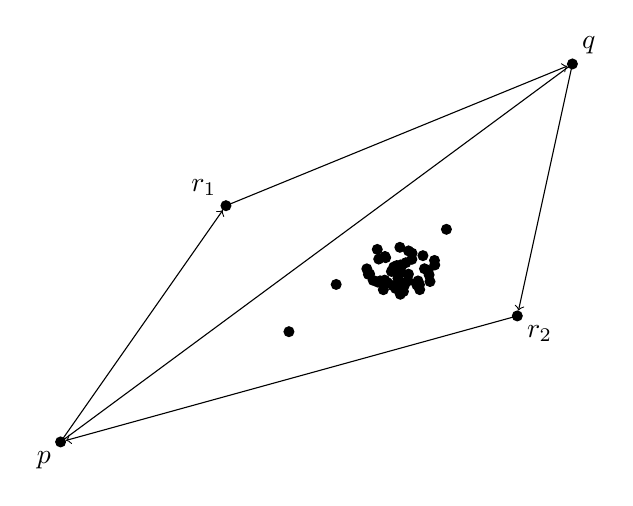
\begin{tikzpicture}
    \fill (0.0, 0.0) coordinate (p) circle (2pt);
    \fill (6.5, 4.8) coordinate (q) circle (2pt);
    \fill (2.1, 3.0) coordinate (rone) circle (2pt);
    \fill (5.8, 1.6) coordinate (rtwo) circle (2pt);

    \node[anchor=north east] at (p) {$p$};
    \node[anchor=south west] at (q) {$q$};
    \node[anchor=south east] at (rone) {$r_1$};
    \node[anchor=north west] at (rtwo) {$r_2$};

    \draw (p) -- (q);
    \draw[->,shorten >=2pt] (p) -- (rone);
    \draw[->,shorten >=2pt] (rone) -- (q);
    \draw[->,shorten >=2pt] (q) -- (rtwo);
    \draw[->,shorten >=2pt] (rtwo) -- (p);

    \pgfmathsetseed{123456}
    \foreach \i in {1,...,50} {
      \pgfmathsetmacro{\ang}{360*rnd}
      \pgfmathsetmacro{\rad}{0.45*sqrt(rnd)}
      \pgfmathsetmacro{\x}{4.3 + 1.05*\rad*cos(\ang)}
      \pgfmathsetmacro{\y}{2.2 + 0.75*\rad*sin(\ang)}
      \fill (\x,\y) circle (2pt);
    }
    \foreach \x/\y in {
      2.9/1.4,
      3.5/2.0,
      4.9/2.7
    } {\fill (\x,\y) circle (2pt);}
  \end{tikzpicture}%
  \caption{The Kuzmin dataset.
  The first partition only moves $r_1$.
  The second partition eliminates all remaining points.}%
  \label{fig:kuzmin}%
\end{figure}

The second dataset consists of points sampled uniformly from a circle, so points of the form $(\cos(\theta), \sin(\theta))$.
A true circle is convex, so all of its points lie on the convex hull.
However, the algorithm finds only \num{10985400} of the $10^8$ points (\qty{\sim11}{\percent}).
This is not a mistake or a problem, because a sampled circle locally resembles a line, up to the square root of the unit round-off, and points on a line can be rejected from the convex hull.
To be more precise, at $(\cos(\theta), \sin(\theta))$, the tangent line has equation
\[
\cos(\theta) x + \sin(\theta) y = 1
\]
The distance between $(\cos(\theta + \delta), \sin(\theta + \delta))$ and this line is
\[
|\cos(\theta)\cos(\theta + \delta) + \sin(\theta + \delta)\sin(\theta) - 1| = \cos(\delta) - 1 = O(\delta^2)
\]
For double precision the unit round-off $u$ is $2^{-53}$, so points on a circle that are approximately $\sqrt{u} \approx 10^{-8}$ apart are indistinguishable from a line and even slight round-off errors create concave points.
Regardless, the recursion is deep and balanced.

The last dataset consists of points sampled uniformly from a disk; the interior of a circle.
The recursion is also balanced, but because we discard more points, the deeper recursion levels are less expensive than for the Circle dataset.

\subsection{Metrics}\label{sec:metrics}
Presenting performance results of an algorithm and its implementation in a meaningful way requires more than the runtime.
The runtime alone tells us little about the quality of the implementation, as we cannot relate it to the capabilities of the machine.
For this reason, we present our results using two statistics.
`'
First\---to evaluate how close the wallclock time gets to the hardware's peak\---we compute the bandwidth, or the amount of data moved divided by time.
We split the $x$- and $y$-coordinates into two separate arrays.
Assuming 64-bit floating\-/point numbers are used, this is $8|P|$ bytes for finding the left\-/most and right\-/most points.
At each recursive call, we have $8(|P| + |S_1| + |S_2|)$ bytes for the partition, and $8|CH(S_2)|$ bytes to place $CH(S_1)$ and $CH(S_2)$ next to each other in memory.
We then scale this by the maximum practical bandwidth of the machine, as measured by the STREAM benchmark (Table~\ref{tab:system}), to get the effective bandwidth utilisation.
Second, we measure the energy consumption in Joules, and use the same approach to compute the energy efficiency in terms of data movement, in \si{\giga\byte\per\joule}.

\subsection{Experimental protocol}
We use GCC 14.1.1.
All experiments are run \num{20} times.
We sweep over the number of threads and over the input size.
For the thread sweep, we fix the input size to $10^8$ points, and vary the number of threads from the sequential case to the number of available threads.
We pick this input size, because the $10^9$ input does not fit in memory on cn125 and laptop for the PBBS implementation.
On the laptop system we use only the performance cores, not the efficiency cores.
For the input size sweep, we fix the number of threads to the maximum available, and vary the input size from $10^5$ to $10^9$ points.
For the bandwidth we plot the mean value and report the error as the standard deviation.
Because energy consumption measurements are not normally distributed and are more susceptible to outliers, we plot the median value and report the error as the interquartile range.
Tables with exact results and a collection of all figures are available in the artefact~\cite{vqhull2025artefact}.

Intel and AMD both provide hardware counters that track the accumulated energy consumption of their processors.
Although initially based on estimation models, these interfaces nowadays provide precise energy consumption statistics~\cite{khan2018rapl}.
Intel CPUs provide these counters since their Sandy Bridge architecture (2011).
AMD started providing them with their Zen architecture (2017).
These counters track the energy consumption of the entire CPU.
The difference between the counter value before and after a benchmark gives the total CPU energy consumed during that benchmark.
Feasibility of measuring system memory is limited by a lack of software interfaces and external power meters, both of which are unavailable to us.

To isolate program\-/induced energy consumption from baseline power draw, across different machines, we subtract the \emph{idle} power draw of the system under
test from the observed energy consumption.
We define idle power draw as the baseline power that is required to keep the hardware operational, as well as the power required for the operating system and additional background tasks.
We measure idle power draw using RAPL counters: across a five\-/minute period, we measure power draw at one\-/second intervals, and take the median value as that hardware's idle power draw.
The hardware on the two cluster systems is fully reserved to ensure that no other tasks are running.
The idle power draw of cn125 was found to be \qty{3.08}{\watt}, and the idle power draw of cn132 was found to be \qty{52.3}{\watt} for the first of the two CPUs, and \qty{50.2}{\watt} for the second.
The difference in power draw between these two nominally identical CPUs is expected, as silicon quality can vary greatly even between CPUs of the same model~\cite{kistowski2016variations}.
Laptop has an idle power draw of \qty{6.26}{\watt}.

\section{Performance evaluation}\label{sec:evaluation}
In this section, we focus on trends in hardware\-/normalised metrics rather than raw throughput and energy consumption.
Specifically, we report bandwidth utilisation and energy efficiency as defined in Section~\ref{sec:metrics}.
These metrics enable meaningful comparisons across systems with different performance characteristics.
Absolute runtime, bandwidth, and energy measurements are provided in the artefact~\cite{vqhull2025artefact}.

To interpret the observed results, we relate differences between VQhull and PBBS to key performance characteristics discussed in Section~\ref{sec:performance}.

\paragraph{Branch prediction}
Branch behaviour differs markedly across datasets.
On Kuzmin, almost all points belong to either $S_1$ or $S_2$, making Hoare's branches highly predictable, which favours PBBS.
VQhull replaces branches with masked SIMD classification, encountering difficult a branch only every \qtyrange{4}{8} elements.
Consequently, PBBS performance varies more with dataset properties, while VQhull tends to be more stable across inputs.

\paragraph{Vectorisation}
SIMD enables VQhull to classify multiple points per operation, achieving more work per instruction than PBBS, even when branch prediction is favourable.
However, speedup does not scale linearly with vector width: the compression instruction itself is not perfectly efficient per element, and other SIMD operations can occur within a single test as well.

\paragraph{Data movement and multithreading}
VQhull combines subset extraction with farthest\-/point search in a single pass, whereas PBBS performs these operations separately.
This increases memory traffic for PBBS, making it more susceptible to bandwidth limitations.

The datasets expose differing amounts of parallel work.
Circle's deep, balanced recursion enables many concurrent sub\-/problems and sustained scaling.
Kuzmin's shallow, unbalanced recursion limits parallelism and amplifies thread management cost.
Disk has balanced recursion but less predictable access patterns, reducing cache locality and prefetch effectiveness.

\begin{figure}[t]
  \scriptsize
  \begin{subfigure}[b]{0.33\linewidth}
    \centering
    \begin{tikzpicture}
\scriptsize
\begin{axis}[
  title={cn125},
  width=\epyfigurewidth,
  height={\epyheightratio*\epyfigurewidth},
  ymin=0,
  xlabel={Threads},
  ylabel={Bandwidth utilization (\si{{\percent}})},
  xmode=log,
  scaled ticks=false,
  xtick={1,2,4,8,16},
  extra y ticks={\pgfkeysvalueof{/pgfplots/ymax}},
  xticklabels={1,2,4,8,16},
  extra y tick labels={\vphantom{Ag}},
  tick pos=left,
  tick align=outside,
  ymajorgrids,
  legend cell align=left,
  major tick length=0.3em,
  /pgf/number format/fixed,
  axis line style={color=black!20},
  y grid style={color=black!20,line width=0.4pt},
  title style={yshift=-1ex},
  tick style={color=black!20,line width=0.4pt},
  tick label style={inner sep=0.15em},
  ylabel style={outer sep=-0.25em},
  extra y tick style={grid=none,major tick length=0pt,yticklabel style={opacity=0,text opacity=0}},
  legend style={draw=black!20,draw opacity=1,fill opacity=0.9,text opacity=1,inner sep=0.2em},
  legend image code/.code={\path[#1] (0em,0pt) -- (1.4em,0pt) plot coordinates {(0.7em,0pt)};},
]
\addplot[draw=none,fill=colorblind0,fill opacity=0.3,forget plot] coordinates {
  (1,46.32527327850714)
  (2,86.30472676434194)
  (4,105.28004815016888)
  (8,126.24515408111516)
  (16,117.88035711247232)
  (16,115.11686450071878)
  (8,124.75714720088298)
  (4,104.69782388074958)
  (2,85.36927854874504)
  (1,46.05686541820134)
} \closedcycle;
\addplot[color=colorblind0,line width=1pt,mark=*,mark size=2pt,mark options={draw=white,line width=-0.4pt,solid}] coordinates {
  (1,46.19106934835424)
  (2,85.83700265654349)
  (4,104.98893601545923)
  (8,125.50115064099907)
  (16,116.49861080659555)
};
\addplot[draw=none,fill=colorblind1,fill opacity=0.3,forget plot] coordinates {
  (1,39.35251415929797)
  (2,69.37530093535898)
  (4,75.74958221214688)
  (8,75.20095008946606)
  (16,61.838755897228474)
  (16,54.701507698108564)
  (8,71.98791064869215)
  (4,74.97440956700056)
  (2,66.66649524311939)
  (1,39.03017055887322)
} \closedcycle;
\addplot[color=colorblind1,line width=1pt,mark=square*,mark size=2pt,mark options={draw=white,line width=-0.4pt,solid}] coordinates {
  (1,39.191342359085596)
  (2,68.02089808923918)
  (4,75.36199588957372)
  (8,73.5944303690791)
  (16,58.27013179766852)
};
\addplot[draw=none,fill=colorblind2,fill opacity=0.3,forget plot] coordinates {
  (1,43.56690382578265)
  (2,74.95086511429379)
  (4,96.29326605440836)
  (8,95.2048642241951)
  (16,83.76381729730926)
  (16,73.51612190327805)
  (8,93.78714675140837)
  (4,93.85533076948396)
  (2,69.9448398840784)
  (1,42.96333964950018)
} \closedcycle;
\addplot[color=colorblind2,line width=1pt,mark=pentagon*,mark size=2pt,mark options={draw=white,line width=-0.4pt,solid}] coordinates {
  (1,43.265121737641415)
  (2,72.4478524991861)
  (4,95.07429841194616)
  (8,94.49600548780174)
  (16,78.63996960029365)
};
\addplot[draw=none,fill=colorblind0,fill opacity=0.3,forget plot] coordinates {
  (1,2.9357214815409285)
  (2,5.218864038228963)
  (4,9.84013686348858)
  (8,17.1412918380299)
  (16,20.334820966366696)
  (16,20.0228486758017)
  (8,16.154447274183333)
  (4,9.784176760300136)
  (2,5.205145190618312)
  (1,2.925599187296488)
} \closedcycle;
\addplot[color=colorblind0,line width=1pt,dashed,mark=*,mark size=2pt,mark options={draw=white,line width=-0.4pt,solid}] coordinates {
  (1,2.9306603344187083)
  (2,5.212004614423638)
  (4,9.812156811894358)
  (8,16.647869556106617)
  (16,20.178834821084198)
};
\addplot[draw=none,fill=colorblind1,fill opacity=0.3,forget plot] coordinates {
  (1,4.570274043709936)
  (2,8.503817467480072)
  (4,16.4110097609223)
  (8,28.150077997815853)
  (16,33.01474067274618)
  (16,32.058905676870204)
  (8,27.326770181890634)
  (4,16.076335477716338)
  (2,8.312827299194584)
  (1,4.560484619364467)
} \closedcycle;
\addplot[color=colorblind1,line width=1pt,dashed,mark=square*,mark size=2pt,mark options={draw=white,line width=-0.4pt,solid}] coordinates {
  (1,4.565379331537201)
  (2,8.408322383337328)
  (4,16.24367261931932)
  (8,27.738424089853243)
  (16,32.53682317480819)
};
\addplot[draw=none,fill=colorblind2,fill opacity=0.3,forget plot] coordinates {
  (1,13.861888698424476)
  (2,18.552236446261553)
  (4,36.38464536396844)
  (8,61.658416155588235)
  (16,58.39593927896554)
  (16,57.90337361992552)
  (8,61.47885097651169)
  (4,36.3572696085591)
  (2,18.54191481498558)
  (1,13.819019617298242)
} \closedcycle;
\addplot[color=colorblind2,line width=1pt,dashed,mark=pentagon*,mark size=2pt,mark options={draw=white,line width=-0.4pt,solid}] coordinates {
  (1,13.840454157861359)
  (2,18.547075630623567)
  (4,36.37095748626377)
  (8,61.56863356604996)
  (16,58.14965644944553)
};
\draw[draw=gray,dashed] (axis cs:8,0) -- (axis cs:8,200);
\end{axis}%
\end{tikzpicture}%%
    \phantomcaption\label{fig:bw-cn125}%
  \end{subfigure}%
  \hfill
  \begin{subfigure}[b]{0.33\linewidth}
    \centering
    \begin{tikzpicture}
\scriptsize
\begin{axis}[
  title={cn132},
  width=\epyfigurewidth,
  height={\epyheightratio*\epyfigurewidth},
  ymin=0,
  xlabel={Threads},
  ylabel={Bandwidth utilization (\si{{\percent}})},
  xmode=log,
  scaled ticks=false,
  xtick={1,2,4,8,16,32},
  extra y ticks={\pgfkeysvalueof{/pgfplots/ymax}},
  xticklabels={1,2,4,8,16,32},
  extra y tick labels={\vphantom{Ag}},
  tick pos=left,
  tick align=outside,
  ymajorgrids,
  legend pos=north west,
  legend cell align=left,
  major tick length=0.3em,
  /pgf/number format/fixed,
  axis line style={color=black!20},
  y grid style={color=black!20,line width=0.4pt},
  title style={yshift=-1ex},
  tick style={color=black!20,line width=0.4pt},
  tick label style={inner sep=0.15em},
  ylabel style={outer sep=-0.25em},
  extra y tick style={grid=none,major tick length=0pt,yticklabel style={opacity=0,text opacity=0}},
  legend style={draw=black!20,draw opacity=1,fill opacity=0.9,text opacity=1,inner sep=0.2em},
  legend image code/.code={\path[#1] (0em,0pt) -- (1.4em,0pt) plot coordinates {(0.7em,0pt)};},
]
\addplot[draw=none,fill=colorblind0,fill opacity=0.3,forget plot] coordinates {
  (1,7.627070022392399)
  (2,16.248588189069583)
  (4,32.57892698711748)
  (8,63.85099750888911)
  (16,114.57844208396448)
  (32,164.53946326257736)
  (32,150.73359245293742)
  (16,112.16782761188337)
  (8,62.840388281870815)
  (4,32.029206772882226)
  (2,15.994478266603007)
  (1,6.823004481741183)
} \closedcycle;
\addplot[color=colorblind0,line width=1pt,mark=*,mark size=2pt,mark options={draw=white,line width=-0.4pt,solid}] coordinates {
  (1,7.225037252066791)
  (2,16.121533227836295)
  (4,32.30406687999985)
  (8,63.34569289537996)
  (16,113.37313484792392)
  (32,157.6365278577574)
};
\addlegendentry{Circle}
\addplot[draw=none,fill=colorblind1,fill opacity=0.3,forget plot] coordinates {
  (1,6.741636665289068)
  (2,13.990463402392864)
  (4,28.401915369647803)
  (8,52.8271976293457)
  (16,77.8473669102587)
  (32,78.46293691454876)
  (32,72.16885093317974)
  (16,73.3165976893676)
  (8,49.574683300250406)
  (4,26.152217073619084)
  (2,12.932835772433412)
  (1,6.021895119311969)
} \closedcycle;
\addplot[color=colorblind1,line width=1pt,mark=square*,mark size=2pt,mark options={draw=white,line width=-0.4pt,solid}] coordinates {
  (1,6.3817658923005185)
  (2,13.461649587413138)
  (4,27.277066221633444)
  (8,51.20094046479805)
  (16,75.58198229981315)
  (32,75.31589392386425)
};
\addlegendentry{Disk}
\addplot[draw=none,fill=colorblind2,fill opacity=0.3,forget plot] coordinates {
  (1,7.351268020715182)
  (2,19.24777971734405)
  (4,35.42000839509254)
  (8,62.16148961648025)
  (16,83.58833120933419)
  (32,85.26675856440193)
  (32,82.85128431200846)
  (16,81.38733139833677)
  (8,57.97932269807235)
  (4,33.83184265177293)
  (2,17.188359438852924)
  (1,6.574498258403636)
} \closedcycle;
\addplot[color=colorblind2,line width=1pt,mark=pentagon*,mark size=2pt,mark options={draw=white,line width=-0.4pt,solid}] coordinates {
  (1,6.962883139559409)
  (2,18.218069578098486)
  (4,34.625925523432734)
  (8,60.0704061572763)
  (16,82.48783130383548)
  (32,84.05902143820519)
};
\addlegendentry{Kuzmin}
\addplot[draw=none,fill=colorblind0,fill opacity=0.3,forget plot] coordinates {
  (1,1.3678662352412623)
  (2,2.0384524413064926)
  (4,4.199144783995001)
  (8,7.216995583885496)
  (16,11.127650124501148)
  (32,15.827366537645291)
  (32,15.65354219190185)
  (16,9.844305267885986)
  (8,6.276888104566734)
  (4,4.13910105665177)
  (2,1.9993939948562638)
  (1,1.306267836624314)
} \closedcycle;
\addplot[color=colorblind0,line width=1pt,dashed,mark=*,mark size=2pt,mark options={draw=white,line width=-0.4pt,solid}] coordinates {
  (1,1.337067035932788)
  (2,2.0189232180813783)
  (4,4.169122920323385)
  (8,6.746941844226115)
  (16,10.485977696193567)
  (32,15.740454364773571)
};
\addplot[draw=none,fill=colorblind1,fill opacity=0.3,forget plot] coordinates {
  (1,1.751581062302018)
  (2,2.8390485883183048)
  (4,5.747218371302671)
  (8,10.90561805761388)
  (16,19.162833317795734)
  (32,27.384634141523986)
  (32,26.372881679734636)
  (16,18.57134687496087)
  (8,10.66742336176027)
  (4,5.593788026825668)
  (2,2.828957885532453)
  (1,1.7195275244272579)
} \closedcycle;
\addplot[color=colorblind1,line width=1pt,dashed,mark=square*,mark size=2pt,mark options={draw=white,line width=-0.4pt,solid}] coordinates {
  (1,1.735554293364638)
  (2,2.834003236925379)
  (4,5.67050319906417)
  (8,10.786520709687075)
  (16,18.867090096378302)
  (32,26.87875791062931)
};
\addplot[draw=none,fill=colorblind2,fill opacity=0.3,forget plot] coordinates {
  (1,7.319400323330377)
  (2,4.1807491894779885)
  (4,8.308484086563196)
  (8,16.392096729901645)
  (16,31.838255320015612)
  (32,55.709314533341406)
  (32,55.05501523426752)
  (16,31.149475151656134)
  (8,16.13521691836891)
  (4,8.195215093597414)
  (2,4.172982365088186)
  (1,6.793849815767463)
} \closedcycle;
\addplot[color=colorblind2,line width=1pt,dashed,mark=pentagon*,mark size=2pt,mark options={draw=white,line width=-0.4pt,solid}] coordinates {
  (1,7.05662506954892)
  (2,4.176865777283087)
  (4,8.251849590080305)
  (8,16.26365682413528)
  (16,31.493865235835873)
  (32,55.382164883804464)
};
\end{axis}%
\end{tikzpicture}%%
    \phantomcaption\label{fig:bw-cn132}%
  \end{subfigure}%
  \hfill
  \begin{subfigure}[b]{0.33\linewidth}
    \centering
    \begin{tikzpicture}
\begin{axis}[
  title={laptop},
  width=\epyfigurewidth,
  height={\epyheightratio*\epyfigurewidth},
  ymin=0,
  xlabel={Threads},
  ylabel={Bandwidth utilization (\si{{\percent}})},
  xmode=log,
  scaled ticks=false,
  xtick={1,2,4,6,12},
  extra y ticks={\pgfkeysvalueof{/pgfplots/ymax}},
  xticklabels={1,2,4,6,12},
  extra y tick labels={\vphantom{Ag}},
  tick pos=left,
  tick align=outside,
  ymajorgrids,
  legend cell align=left,
  major tick length=0.3em,
  /pgf/number format/fixed,
  axis line style={color=black!20},
  y grid style={color=black!20,line width=0.4pt},
  tick style={color=black!20,line width=0.4pt},
  tick label style={inner sep=0.15em},
  ylabel style={outer sep=-0.25em},
  extra y tick style={grid=none,major tick length=0pt,yticklabel style={opacity=0,text opacity=0}},
  legend style={draw=black!20,draw opacity=1,fill opacity=0.9,text opacity=1,inner sep=0.2em},
  legend image code/.code={\path[#1] (0em,0pt) -- (1.4em,0pt) plot coordinates {(0.7em,0pt)};},
]
\addplot[draw=none,fill=colorblind0,fill opacity=0.3,forget plot] coordinates {
  (1,32.484831403554885)
  (2,62.53168595377395)
  (4,80.64791175659012)
  (6,88.1992876002579)
  (12,100.10265715696993)
  (12,97.32429518157763)
  (6,86.37086129468939)
  (4,80.37685353045067)
  (2,61.46401915467336)
  (1,31.65400713806209)
} \closedcycle;
\addplot[color=colorblind0,line width=1pt,mark=*,mark size=2pt,mark options={draw=white,line width=-0.4pt,solid}] coordinates {
  (1,32.06941927080849)
  (2,61.997852554223655)
  (4,80.5123826435204)
  (6,87.28507444747365)
  (12,98.71347616927378)
};
\addplot[draw=none,fill=colorblind1,fill opacity=0.3,forget plot] coordinates {
  (1,30.06856681795748)
  (2,52.18629296015595)
  (4,65.79004220957009)
  (6,81.53385367095537)
  (12,88.90432658819644)
  (12,84.56078072719613)
  (6,80.60191293050737)
  (4,64.89279007535902)
  (2,47.37667463804455)
  (1,25.98713247247669)
} \closedcycle;
\addplot[color=colorblind1,line width=1pt,mark=square*,mark size=2pt,mark options={draw=white,line width=-0.4pt,solid}] coordinates {
  (1,28.027849645217085)
  (2,49.78148379910025)
  (4,65.34141614246455)
  (6,81.06788330073137)
  (12,86.73255365769629)
};
\addplot[draw=none,fill=colorblind2,fill opacity=0.3,forget plot] coordinates {
  (1,37.49361584187408)
  (2,60.52199717956696)
  (4,88.90290250500976)
  (6,100.98162534992127)
  (12,106.51080111686483)
  (12,101.99244033930344)
  (6,98.56632704426079)
  (4,83.17264011544393)
  (2,53.25705701881265)
  (1,32.20609780242412)
} \closedcycle;
\addplot[color=colorblind2,line width=1pt,mark=pentagon*,mark size=2pt,mark options={draw=white,line width=-0.4pt,solid}] coordinates {
  (1,34.8498568221491)
  (2,56.889527099189806)
  (4,86.03777131022684)
  (6,99.77397619709103)
  (12,104.25162072808413)
};
\addplot[draw=none,fill=colorblind0,fill opacity=0.3,forget plot] coordinates {
  (1,4.85523253740951)
  (2,7.513960190431021)
  (4,13.446030539655544)
  (6,16.89867867642413)
  (12,19.617536307901187)
  (12,18.540076835756768)
  (6,16.296331160920513)
  (4,12.906403547570159)
  (2,7.280350621029262)
  (1,4.621657741075744)
} \closedcycle;
\addplot[color=colorblind0,line width=1pt,dashed,mark=*,mark size=2pt,mark options={draw=white,line width=-0.4pt,solid}] coordinates {
  (1,4.738445139242627)
  (2,7.397155405730142)
  (4,13.176217043612851)
  (6,16.59750491867232)
  (12,19.078806571828977)
};
\addplot[draw=none,fill=colorblind1,fill opacity=0.3,forget plot] coordinates {
  (1,6.553032530990638)
  (2,10.596088839279147)
  (4,17.774445578957824)
  (6,24.689040373365692)
  (12,29.04453277298816)
  (12,28.2232018046082)
  (6,22.462870536282153)
  (4,17.42496097002067)
  (2,9.899855897855453)
  (1,6.465139281233032)
} \closedcycle;
\addplot[color=colorblind1,line width=1pt,dashed,mark=square*,mark size=2pt,mark options={draw=white,line width=-0.4pt,solid}] coordinates {
  (1,6.509085906111835)
  (2,10.2479723685673)
  (4,17.599703274489247)
  (6,23.575955454823923)
  (12,28.63386728879818)
};
\addplot[draw=none,fill=colorblind2,fill opacity=0.3,forget plot] coordinates {
  (1,19.834586367531553)
  (2,27.28388620759916)
  (4,48.83333834846525)
  (6,64.98920659294762)
  (12,71.70836484057673)
  (12,62.85701907321416)
  (6,61.86545985598971)
  (4,44.82745056437628)
  (2,26.475382439948348)
  (1,17.318315169827496)
} \closedcycle;
\addplot[color=colorblind2,line width=1pt,dashed,mark=pentagon*,mark size=2pt,mark options={draw=white,line width=-0.4pt,solid}] coordinates {
  (1,18.576450768679525)
  (2,26.879634323773754)
  (4,46.83039445642076)
  (6,63.42733322446867)
  (12,67.28269195689545)
};
\draw[draw=gray,dashed] (axis cs:6,0) -- (axis cs:6,200);
\end{axis}
\end{tikzpicture}%
    \phantomcaption\label{fig:bw-laptop}%
  \end{subfigure}%
  \caption{Bandwidth utilisation for $10^8$ points, as a percentage of STREAM's bandwidth.
  The solid lines represent the VQhull implementation, the dashed lines represent the PBBS implementation.
  Each dataset is shown with a unique colour and marker.}%
  \label{fig:bw}%
\end{figure}

\subsection{Throughput scaling with thread count}
Figure~\ref{fig:bw} shows bandwidth utilisation for $10^8$ points as a function of thread count, normalised to STREAM bandwidth.
Utilisation above \qty{100}{\percent} can occur when deeper recursion levels operate on subsets that fit in cache, reducing the need to access main memory.

For VQhull, Circle scales best on cn125 and cn132.
Circle's deep and balanced recursion enables more parallel work at deeper levels.
On cn125, bandwidth utilisation peaks around \qty{125}{\percent} at eight threads and then drops slightly with multithreading.
On cn132, performance continues to improve up to 32 threads.
Disk consistently underperforms Circle and Kuzmin.
This can be attributed to less predictable access patterns, which reduce the effectiveness of hardware prefetching and lower cache efficiency.
On cn132, scaling is further affected by the dual\-/socket architecture.
Recursive tasks may be scheduled on different sockets, increasing the likelihood of remote memory accesses and reducing effective bandwidth.

For Kuzmin, VQhull achieves close to full STREAM bandwidth on non\-/NUMA systems but only \qty{\sim80}{\percent} on cn132.
Profiling reveals that initial subset extraction reaches full bandwidth, but deeper recursions suffer from suboptimal thread placement across sockets, which we do not control.

The laptop's larger per\-/core L2 cache (Table~\ref{tab:system}) reduces cache misses, which consequently lowers pressure on main memory.
This particularly benefits Kuzmin and Disk, whose performance is otherwise more sensitive to memory access patterns, and explains why their performance approaches that of Circle on this system.

PBBS exhibits weaker parallel scaling.
Multiple passes over the data increase memory traffic, and sparse subsets at deeper levels reduce cacheline efficiency for Circle and Disk.
Consequently, PBBS performs relatively better on Kuzmin, where memory access patterns are more predictable.

\begin{figure}[t]
  \scriptsize
  \begin{subfigure}[b]{0.33\linewidth}
    \centering
    \begin{tikzpicture}
\begin{axis}[
  title={cn125},
  width=\epyfigurewidth,
  height={\epyheightratio*\epyfigurewidth},
  ymin=0,
  xlabel={Input size (points)},
  ylabel={Bandwidth utilization (\si{{\percent}})},
  xmode=log,
  scaled ticks=false,
  xtick={100000,1000000,10000000,100000000,1000000000},
  extra y ticks={\pgfkeysvalueof{/pgfplots/ymax}},
  extra y tick labels={\vphantom{Ag}},
  tick pos=left,
  tick align=outside,
  ymajorgrids,
  legend cell align=left,
  major tick length=0.3em,
  /pgf/number format/fixed,
  axis line style={color=black!20},
  y grid style={color=black!20,line width=0.4pt},
  tick style={color=black!20,line width=0.4pt},
  tick label style={inner sep=0.15em},
  ylabel style={outer sep=-0.25em},
  extra y tick style={grid=none,major tick length=0pt,yticklabel style={opacity=0,text opacity=0}},
  legend style={draw=black!20,draw opacity=1,fill opacity=0.9,text opacity=1,inner sep=0.2em},
  legend image code/.code={\path[#1] (0em,0pt) -- (1.4em,0pt) plot coordinates {(0.7em,0pt)};},
]
\addplot[draw=none,fill=colorblind0,fill opacity=0.3,forget plot] coordinates {
  (100000,10.59838990844274)
  (1000000,25.010175164791637)
  (10000000,89.95762076662604)
  (100000000,120.3579674290643)
  (1000000000,109.11645092804427)
  (1000000000,108.22562906086766)
  (100000000,116.99847889018702)
  (10000000,83.2648318699404)
  (1000000,19.069903604820308)
  (100000,6.595851787274451)
} \closedcycle;
\addplot[color=colorblind0,line width=1pt,mark=*,mark size=2pt,mark options={draw=white,line width=-0.4pt,solid}] coordinates {
  (100000,8.597120847858596)
  (1000000,22.040039384805972)
  (10000000,86.61122631828322)
  (100000000,118.67822315962566)
  (1000000000,108.67103999445597)
};
\addplot[draw=none,fill=colorblind1,fill opacity=0.3,forget plot] coordinates {
  (100000,1.244099927722852)
  (1000000,2.8712141534996802)
  (10000000,19.963637538223686)
  (100000000,66.03091200197035)
  (1000000000,75.63591453228142)
  (1000000000,73.83158460212167)
  (100000000,58.41502022480751)
  (10000000,14.547699315042292)
  (1000000,2.194960116716319)
  (100000,0.6781624185700696)
} \closedcycle;
\addplot[color=colorblind1,line width=1pt,mark=square*,mark size=2pt,mark options={draw=white,line width=-0.4pt,solid}] coordinates {
  (100000,0.9611311731464608)
  (1000000,2.5330871351079995)
  (10000000,17.25566842663299)
  (100000000,62.222966113388935)
  (1000000000,74.73374956720154)
};
\addplot[draw=none,fill=colorblind2,fill opacity=0.3,forget plot] coordinates {
  (100000,25.244977242300607)
  (1000000,56.811373815906144)
  (10000000,72.63699032045801)
  (100000000,88.61606622988985)
  (1000000000,87.58760947633269)
  (1000000000,84.54760204353414)
  (100000000,86.00195414399549)
  (10000000,71.52050682901736)
  (1000000,48.899521427069764)
  (100000,23.836124842048626)
} \closedcycle;
\addplot[color=colorblind2,line width=1pt,mark=pentagon*,mark size=2pt,mark options={draw=white,line width=-0.4pt,solid}] coordinates {
  (100000,24.540551042174616)
  (1000000,52.855447621487954)
  (10000000,72.07874857473769)
  (100000000,87.30901018694267)
  (1000000000,86.06760575993341)
};
\addplot[draw=none,fill=colorblind0,fill opacity=0.3,forget plot] coordinates {
  (100000,23.615434628003666)
  (1000000,24.54923576464996)
  (10000000,22.6768993078029)
  (100000000,20.443175950664692)
  (100000000,20.12385175961457)
  (10000000,21.610632216281395)
  (1000000,23.924392889424038)
  (100000,21.882115003443932)
} \closedcycle;
\addplot[color=colorblind0,line width=1pt,dashed,mark=*,mark size=2pt,mark options={draw=white,line width=-0.4pt,solid}] coordinates {
  (100000,22.7487748157238)
  (1000000,24.236814327037)
  (10000000,22.143765762042147)
  (100000000,20.28351385513963)
};
\addplot[draw=none,fill=colorblind1,fill opacity=0.3,forget plot] coordinates {
  (100000,38.05388026110748)
  (1000000,40.515605050606794)
  (10000000,33.71331495631996)
  (100000000,33.10200552338219)
  (100000000,32.003770952175046)
  (10000000,32.06940119329957)
  (1000000,39.50829823068375)
  (100000,20.158707817333983)
} \closedcycle;
\addplot[color=colorblind1,line width=1pt,dashed,mark=square*,mark size=2pt,mark options={draw=white,line width=-0.4pt,solid}] coordinates {
  (100000,29.10629403922073)
  (1000000,40.01195164064527)
  (10000000,32.891358074809766)
  (100000000,32.55288823777862)
};
\addplot[draw=none,fill=colorblind2,fill opacity=0.3,forget plot] coordinates {
  (100000,62.82416339617754)
  (1000000,71.9695938365408)
  (10000000,58.91256491072156)
  (100000000,58.353641083575866)
  (100000000,58.180431132609186)
  (10000000,57.10881785296495)
  (1000000,62.17532868693628)
  (100000,57.78625728904207)
} \closedcycle;
\addplot[color=colorblind2,line width=1pt,dashed,mark=pentagon*,mark size=2pt,mark options={draw=white,line width=-0.4pt,solid}] coordinates {
  (100000,60.305210342609804)
  (1000000,67.07246126173854)
  (10000000,58.01069138184325)
  (100000000,58.267036108092526)
};
\end{axis}%
\end{tikzpicture}%%
    \phantomcaption\label{fig:points-cn125}%
  \end{subfigure}%
  \hfill
  \begin{subfigure}[b]{0.33\linewidth}
    \centering
    \begin{tikzpicture}
\scriptsize
\begin{axis}[
  title={cn132},
  width=\epyfigurewidth,
  height={\epyheightratio*\epyfigurewidth},
  ymin=0,
  xlabel={Input size (points)},
  ylabel={Bandwidth utilization (\si{{\percent}})},
  xmode=log,
  scaled ticks=false,
  xtick={100000,1000000,10000000,100000000,1000000000},
  extra y ticks={\pgfkeysvalueof{/pgfplots/ymax}},
  extra y tick labels={\vphantom{Ag}},
  tick pos=left,
  tick align=outside,
  ymajorgrids,
  legend pos=north west,
  legend cell align=left,
  major tick length=0.3em,
  /pgf/number format/fixed,
  axis line style={color=black!20},
  y grid style={color=black!20,line width=0.4pt},
  title style={yshift=-1ex},
  tick style={color=black!20,line width=0.4pt},
  tick label style={inner sep=0.15em},
  ylabel style={outer sep=-0.25em},
  extra y tick style={grid=none,major tick length=0pt,yticklabel style={opacity=0,text opacity=0}},
  legend style={draw=black!20,draw opacity=1,fill opacity=0.9,text opacity=1,inner sep=0.2em},
  legend image code/.code={\path[#1] (0em,0pt) -- (1.4em,0pt) plot coordinates {(0.7em,0pt)};},
]
\addplot[draw=none,fill=colorblind0,fill opacity=0.3,forget plot] coordinates {
  (100000,12.800188566628758)
  (1000000,39.55735755959984)
  (10000000,121.59097001241048)
  (100000000,160.43709207583683)
  (1000000000,150.09385663827987)
  (1000000000,146.89406603478136)
  (100000000,157.56992697288646)
  (10000000,113.1872107053401)
  (1000000,23.149847167842744)
  (100000,11.45273044325339)
} \closedcycle;
\addplot[color=colorblind0,line width=1pt,mark=*,mark size=2pt,mark options={draw=white,line width=-0.4pt,solid}] coordinates {
  (100000,12.126459504941074)
  (1000000,31.353602363721294)
  (10000000,117.3890903588753)
  (100000000,159.00350952436165)
  (1000000000,148.49396133653062)
};
\addlegendentry{Circle}
\addplot[draw=none,fill=colorblind1,fill opacity=0.3,forget plot] coordinates {
  (100000,0.3743103035411093)
  (1000000,3.853500365844502)
  (10000000,34.63895231784267)
  (100000000,77.3352493333508)
  (1000000000,87.8190987263642)
  (1000000000,85.92279759001208)
  (100000000,75.15340347369063)
  (10000000,30.69339340424941)
  (1000000,2.611455102485167)
  (100000,0.24571585409322194)
} \closedcycle;
\addplot[color=colorblind1,line width=1pt,mark=square*,mark size=2pt,mark options={draw=white,line width=-0.4pt,solid}] coordinates {
  (100000,0.3100130788171656)
  (1000000,3.2324777341648345)
  (10000000,32.66617286104604)
  (100000000,76.24432640352072)
  (1000000000,86.87094815818814)
};
\addlegendentry{Disk}
\addplot[draw=none,fill=colorblind2,fill opacity=0.3,forget plot] coordinates {
  (100000,2.8001796371518006)
  (1000000,6.119886808170244)
  (10000000,47.4925023152459)
  (100000000,84.43825988556559)
  (1000000000,97.1770573618142)
  (1000000000,94.60758333039686)
  (100000000,81.57249444600363)
  (10000000,39.71419629414042)
  (1000000,5.907336790289837)
  (100000,2.6322487405771273)
} \closedcycle;
\addplot[color=colorblind2,line width=1pt,mark=pentagon*,mark size=2pt,mark options={draw=white,line width=-0.4pt,solid}] coordinates {
  (100000,2.716214188864464)
  (1000000,6.01361179923004)
  (10000000,43.60334930469316)
  (100000000,83.00537716578461)
  (1000000000,95.89232034610554)
};
\addlegendentry{Kuzmin}
\addplot[draw=none,fill=colorblind0,fill opacity=0.3,forget plot] coordinates {
  (100000,11.072353859185002)
  (1000000,25.95839236434012)
  (10000000,15.913948555943016)
  (100000000,16.032014993337366)
  (1000000000,14.051472413295114)
  (1000000000,13.950589590001252)
  (100000000,15.851222416896306)
  (10000000,15.329826195282394)
  (1000000,23.821864851178404)
  (100000,8.65444838107055)
} \closedcycle;
\addplot[color=colorblind0,line width=1pt,dashed,mark=*,mark size=2pt,mark options={draw=white,line width=-0.4pt,solid}] coordinates {
  (100000,9.863401120127776)
  (1000000,24.890128607759262)
  (10000000,15.621887375612705)
  (100000000,15.941618705116836)
  (1000000000,14.001031001648183)
};
\addplot[draw=none,fill=colorblind1,fill opacity=0.3,forget plot] coordinates {
  (100000,6.89519928325105)
  (1000000,32.566766290711804)
  (10000000,12.337835256321174)
  (100000000,27.580565271556445)
  (1000000000,34.84935260484607)
  (1000000000,34.303846665740046)
  (100000000,25.761965183436573)
  (10000000,11.503429330768633)
  (1000000,23.71492844948802)
  (100000,5.974026466540747)
} \closedcycle;
\addplot[color=colorblind1,line width=1pt,dashed,mark=square*,mark size=2pt,mark options={draw=white,line width=-0.4pt,solid}] coordinates {
  (100000,6.434612874895898)
  (1000000,28.140847370099912)
  (10000000,11.920632293544903)
  (100000000,26.67126522749651)
  (1000000000,34.57659963529306)
};
\addplot[draw=none,fill=colorblind2,fill opacity=0.3,forget plot] coordinates {
  (100000,8.968801843590539)
  (1000000,21.37022887803655)
  (10000000,20.046074703545656)
  (100000000,55.6663669172884)
  (1000000000,56.69041141476958)
  (1000000000,56.51369595807778)
  (100000000,54.64531626077601)
  (10000000,18.966140138885187)
  (1000000,19.34386225076772)
  (100000,8.128890773434941)
} \closedcycle;
\addplot[color=colorblind2,line width=1pt,dashed,mark=pentagon*,mark size=2pt,mark options={draw=white,line width=-0.4pt,solid}] coordinates {
  (100000,8.54884630851274)
  (1000000,20.357045564402135)
  (10000000,19.50610742121542)
  (100000000,55.15584158903221)
  (1000000000,56.60205368642368)
};
\end{axis}%
\end{tikzpicture}%%
    \phantomcaption\label{fig:points-cn132}%
  \end{subfigure}%
  \hfill
  \begin{subfigure}[b]{0.33\linewidth}
    \centering
    \begin{tikzpicture}
\begin{axis}[
  title={laptop},
  width=\epyfigurewidth,
  height={\epyheightratio*\epyfigurewidth},
  ymin=0,
  xlabel={Input size (points)},
  ylabel={Bandwidth utilization (\si{{\percent}})},
  xmode=log,
  scaled ticks=false,
  xtick={100000,1000000,10000000,100000000,1000000000},
  extra y ticks={\pgfkeysvalueof{/pgfplots/ymax}},
  extra y tick labels={\vphantom{Ag}},
  tick pos=left,
  tick align=outside,
  ymajorgrids,
  legend cell align=left,
  major tick length=0.3em,
  /pgf/number format/fixed,
  axis line style={color=black!20},
  y grid style={color=black!20,line width=0.4pt},
  tick style={color=black!20,line width=0.4pt},
  tick label style={inner sep=0.15em},
  ylabel style={outer sep=-0.25em},
  extra y tick style={grid=none,major tick length=0pt,yticklabel style={opacity=0,text opacity=0}},
  legend style={draw=black!20,draw opacity=1,fill opacity=0.9,text opacity=1,inner sep=0.2em},
  legend image code/.code={\path[#1] (0em,0pt) -- (1.4em,0pt) plot coordinates {(0.7em,0pt)};},
]
\addplot[draw=none,fill=colorblind0,fill opacity=0.3,forget plot] coordinates {
  (100000,47.04183047982237)
  (1000000,95.64175127891542)
  (10000000,94.29367321659366)
  (100000000,109.22229042230371)
  (1000000000,105.17550131553412)
  (1000000000,90.12170162549913)
  (100000000,92.81285714498604)
  (10000000,89.942359427179)
  (1000000,75.55213330197856)
  (100000,34.92193257802817)
} \closedcycle;
\addplot[color=colorblind0,line width=1pt,mark=*,mark size=2pt,mark options={draw=white,line width=-0.4pt,solid}] coordinates {
  (100000,40.98188152892527)
  (1000000,85.59694229044699)
  (10000000,92.11801632188633)
  (100000000,101.01757378364488)
  (1000000000,97.64860147051662)
};
\addplot[draw=none,fill=colorblind1,fill opacity=0.3,forget plot] coordinates {
  (100000,8.822462001496552)
  (1000000,44.07426678443832)
  (10000000,78.33188470866209)
  (100000000,87.83398264912728)
  (1000000000,91.21537629503305)
  (1000000000,89.09095021773314)
  (100000000,83.73998601590347)
  (10000000,68.67716041663071)
  (1000000,32.8585104180532)
  (100000,5.109072417410537)
} \closedcycle;
\addplot[color=colorblind1,line width=1pt,mark=square*,mark size=2pt,mark options={draw=white,line width=-0.4pt,solid}] coordinates {
  (100000,6.965767209453545)
  (1000000,38.46638860124576)
  (10000000,73.5045225626464)
  (100000000,85.78698433251537)
  (1000000000,90.1531632563831)
};
\addplot[draw=none,fill=colorblind2,fill opacity=0.3,forget plot] coordinates {
  (100000,13.38222771276498)
  (1000000,59.415892042977106)
  (10000000,97.85375114900083)
  (100000000,106.88003836339672)
  (1000000000,111.87485331757372)
  (1000000000,106.7264678763506)
  (100000000,101.01146848020753)
  (10000000,80.8191591708937)
  (1000000,46.63653834480742)
  (100000,8.682081043651003)
} \closedcycle;
\addplot[color=colorblind2,line width=1pt,mark=pentagon*,mark size=2pt,mark options={draw=white,line width=-0.4pt,solid}] coordinates {
  (100000,11.032154378207991)
  (1000000,53.02621519389226)
  (10000000,89.33645515994726)
  (100000000,103.94575342180212)
  (1000000000,109.30066059696216)
};
\addplot[draw=none,fill=colorblind0,fill opacity=0.3,forget plot] coordinates {
  (100000,27.339285196469486)
  (1000000,29.257600121326924)
  (10000000,22.873339494954617)
  (100000000,18.895870217699144)
  (100000000,17.127617431981836)
  (10000000,20.1425721126132)
  (1000000,26.3200425542896)
  (100000,22.185104413077052)
} \closedcycle;
\addplot[color=colorblind0,line width=1pt,dashed,mark=*,mark size=2pt,mark options={draw=white,line width=-0.4pt,solid}] coordinates {
  (100000,24.76219480477327)
  (1000000,27.788821337808262)
  (10000000,21.507955803783908)
  (100000000,18.01174382484049)
};
\addplot[draw=none,fill=colorblind1,fill opacity=0.3,forget plot] coordinates {
  (100000,33.76420780774549)
  (1000000,38.005848048854396)
  (10000000,31.27662325992016)
  (100000000,26.902793548396563)
  (100000000,25.32221703659626)
  (10000000,28.98822171920583)
  (1000000,30.19523905248834)
  (100000,28.213639803740264)
} \closedcycle;
\addplot[color=colorblind1,line width=1pt,dashed,mark=square*,mark size=2pt,mark options={draw=white,line width=-0.4pt,solid}] coordinates {
  (100000,30.98892380574288)
  (1000000,34.10054355067137)
  (10000000,30.132422489562995)
  (100000000,26.11250529249641)
};
\addplot[draw=none,fill=colorblind2,fill opacity=0.3,forget plot] coordinates {
  (100000,58.99491467840087)
  (1000000,70.17148609653687)
  (10000000,67.64231332117741)
  (100000000,62.25575750689544)
  (100000000,60.92128495371775)
  (10000000,52.20636928763799)
  (1000000,53.79876979967048)
  (100000,46.36357801906423)
} \closedcycle;
\addplot[color=colorblind2,line width=1pt,dashed,mark=pentagon*,mark size=2pt,mark options={draw=white,line width=-0.4pt,solid}] coordinates {
  (100000,52.67924634873255)
  (1000000,61.985127948103674)
  (10000000,59.924341304407704)
  (100000000,61.5885212303066)
};
\end{axis}%
\end{tikzpicture}%%
    \phantomcaption\label{fig:points-laptop}%
  \end{subfigure}%
  \caption{Bandwidth utilisation over input sweep as a percentage of STREAM's bandwidth, fixed at the maximum number of available threads.
  The solid lines represent the VQhull implementation, the dashed lines represent the PBBS implementation.
  Each dataset is shown with a unique colour and marker.}%
  \label{fig:points}%
\end{figure}

\subsection{Throughput scaling with input size}
Figure~\ref{fig:points} shows bandwidth utilisation as a function of input size from $10^5$ to $10^9$ points (\qty{1.6}{\mega\byte}--\qty{16}{\giga\byte}), using the maximum number of threads on each system.
For the largest input size, PBBS results are missing on cn125 and laptop.
PBBS partitions an array of indices instead of the points themselves, resulting in a higher memory footprint that exceeds the hardware capabilities on those systems.

For small inputs, PBBS achieves higher bandwidth utilisation than VQhull because VQhull's overhead from alignment, block\-/cyclic distribution, and thread balancing has not yet amortized.
As input size increases, VQhull performance improves rapidly until saturation occurs at memory bandwidth.
The saturation point depends on both the dataset and system.
On cn132, NUMA effects dominate at larger sizes, causing Disk and Kuzmin to exhibit similar scaling despite their structural differences.

\begin{figure}[t]
  \scriptsize
  \begin{subfigure}[b]{0.33\linewidth}
    \centering
    \begin{tikzpicture}
\scriptsize
\begin{axis}[
  title={cn125},
  width=\epyfigurewidth,
  height={\epyheightratio*\epyfigurewidth},
  ymin=0,
  xlabel={Threads},
  ylabel={Energy efficiency (\si{\giga\byte\per\joule})},
  xmode=log,
  scaled ticks=false,
  xtick={1,2,4,8,16},
  extra y ticks={\pgfkeysvalueof{/pgfplots/ymax}},
  xticklabels={1,2,4,8,16},
  extra y tick labels={\vphantom{Ag}},
  tick pos=left,
  tick align=outside,
  ymajorgrids,
  legend cell align=left,
  major tick length=0.3em,
  /pgf/number format/fixed,
  axis line style={color=black!20},
  y grid style={color=black!20,line width=0.4pt},
  title style={yshift=-1ex},
  tick style={color=black!20,line width=0.4pt},
  tick label style={inner sep=0.15em},
  ylabel style={outer sep=-0.25em},
  extra y tick style={grid=none,major tick length=0pt,yticklabel style={opacity=0,text opacity=0}},
  legend style={draw=black!20,draw opacity=1,fill opacity=0.9,text opacity=1,inner sep=0.2em},
  legend image code/.code={\path[#1] (0em,0pt) -- (1.4em,0pt) plot coordinates {(0.7em,0pt)};},
]
\addplot[draw=none,fill=colorblind0,fill opacity=0.3,forget plot] coordinates {
  (1,1.276329018558754)
  (2,1.7061680994574355)
  (4,1.7975224253337512)
  (8,1.7710066726891671)
  (16,1.5506948631146407)
  (16,1.5361635159664162)
  (8,1.7592530134368172)
  (4,1.786577158685364)
  (2,1.6868413649453255)
  (1,1.2563937554108533)
} \closedcycle;
\addplot[color=colorblind0,line width=1pt,mark=*,mark size=2pt,mark options={draw=white,line width=-0.4pt,solid}] coordinates {
  (1,1.2681008425626707)
  (2,1.7016412341749874)
  (4,1.79327485085601)
  (8,1.7676881609151711)
  (16,1.5449700166006946)
};
\addplot[draw=none,fill=colorblind1,fill opacity=0.3,forget plot] coordinates {
  (1,1.029491541646957)
  (2,1.302876546801578)
  (4,1.1684814568107387)
  (8,0.8723319885914709)
  (16,0.6647497669412863)
  (16,0.6390488706042714)
  (8,0.858195588856299)
  (4,1.1401191590918773)
  (2,1.2683985481082627)
  (1,1.0200781695568322)
} \closedcycle;
\addplot[color=colorblind1,line width=1pt,mark=square*,mark size=2pt,mark options={draw=white,line width=-0.4pt,solid}] coordinates {
  (1,1.0258425214619042)
  (2,1.282355169912956)
  (4,1.16404283974348)
  (8,0.8686314175636622)
  (16,0.6496852318233329)
};
\addplot[draw=none,fill=colorblind2,fill opacity=0.3,forget plot] coordinates {
  (1,1.1639332416143655)
  (2,1.4060036570663286)
  (4,1.3453800228383395)
  (8,0.933804619032839)
  (16,0.8024673541848344)
  (16,0.790321440413323)
  (8,0.928163584334095)
  (4,1.3224586565597338)
  (2,1.3615927415487719)
  (1,1.1530764036440095)
} \closedcycle;
\addplot[color=colorblind2,line width=1pt,mark=pentagon*,mark size=2pt,mark options={draw=white,line width=-0.4pt,solid}] coordinates {
  (1,1.1592327806996183)
  (2,1.4012054012524304)
  (4,1.337017076201755)
  (8,0.9294649212500365)
  (16,0.7939174042591903)
};
\addplot[draw=none,fill=colorblind0,fill opacity=0.3,forget plot] coordinates {
  (1,0.08923755554908293)
  (2,0.13138149754328332)
  (4,0.17505366496471275)
  (8,0.1927026135840852)
  (16,0.2200634032411107)
  (16,0.21724481162844797)
  (8,0.18945365456938726)
  (4,0.17384462554250396)
  (2,0.12991482780518568)
  (1,0.08772676830827511)
} \closedcycle;
\addplot[color=colorblind0,line width=1pt,dashed,mark=*,mark size=2pt,mark options={draw=white,line width=-0.4pt,solid}] coordinates {
  (1,0.08896579671787283)
  (2,0.13109437687449188)
  (4,0.17441296557698674)
  (8,0.19157226328396026)
  (16,0.21880118545775745)
};
\addplot[draw=none,fill=colorblind1,fill opacity=0.3,forget plot] coordinates {
  (1,0.13801683584089305)
  (2,0.21497782141674943)
  (4,0.2868433459055822)
  (8,0.3173214350701123)
  (16,0.3544855424177959)
  (16,0.3502319322911483)
  (8,0.31338376258853773)
  (4,0.2736815132659659)
  (2,0.21096606923797473)
  (1,0.13552126215396187)
} \closedcycle;
\addplot[color=colorblind1,line width=1pt,dashed,mark=square*,mark size=2pt,mark options={draw=white,line width=-0.4pt,solid}] coordinates {
  (1,0.13714615126743213)
  (2,0.21371976129649864)
  (4,0.2844409693098223)
  (8,0.314316541253162)
  (16,0.3525588123344852)
};
\addplot[draw=none,fill=colorblind2,fill opacity=0.3,forget plot] coordinates {
  (1,0.41957488321453196)
  (2,0.4553740710610309)
  (4,0.6096557800442406)
  (8,0.6573442200223013)
  (16,0.5945267445271327)
  (16,0.5930528347612725)
  (8,0.6549485272625835)
  (4,0.6076646010989555)
  (2,0.4534286643066389)
  (1,0.41763522641841494)
} \closedcycle;
\addplot[color=colorblind2,line width=1pt,dashed,mark=pentagon*,mark size=2pt,mark options={draw=white,line width=-0.4pt,solid}] coordinates {
  (1,0.4188209605265828)
  (2,0.45476689380305635)
  (4,0.6089259877696434)
  (8,0.6560617535285747)
  (16,0.593543928071147)
};
\draw[draw=gray,dashed] (axis cs:8,0) -- (axis cs:8,5);
\end{axis}%
\end{tikzpicture}%%
    \phantomcaption\label{fig:energy-cn125}%
  \end{subfigure}%
  \hfill
  \begin{subfigure}[b]{0.33\linewidth}
    \centering
    \begin{tikzpicture}
\scriptsize
\begin{axis}[
  title={cn132},
  width=\epyfigurewidth,
  height={\epyheightratio*\epyfigurewidth},
  ymin=0,
  xlabel={Threads},
  ylabel={Energy efficiency (\si{\giga\byte\per\joule})},
  xmode=log,
  scaled ticks=false,
  xtick={1,2,4,8,16,32},
  extra y ticks={\pgfkeysvalueof{/pgfplots/ymax}},
  xticklabels={1,2,4,8,16,32},
  extra y tick labels={\vphantom{Ag}},
  tick pos=left,
  tick align=outside,
  ymajorgrids,
  legend pos=north west,
  legend cell align=left,
  major tick length=0.3em,
  /pgf/number format/fixed,
  axis line style={color=black!20},
  y grid style={color=black!20,line width=0.4pt},
  title style={yshift=-1ex},
  tick style={color=black!20,line width=0.4pt},
  tick label style={inner sep=0.15em},
  ylabel style={outer sep=-0.25em},
  extra y tick style={grid=none,major tick length=0pt,yticklabel style={opacity=0,text opacity=0}},
  legend style={draw=black!20,draw opacity=1,fill opacity=0.9,text opacity=1,inner sep=0.2em},
  legend image code/.code={\path[#1] (0em,0pt) -- (1.4em,0pt) plot coordinates {(0.7em,0pt)};},
]
\addplot[draw=none,fill=colorblind0,fill opacity=0.3,forget plot] coordinates {
  (1,0.5341751098692948)
  (2,0.45611212915098437)
  (4,0.6980792303848139)
  (8,0.9251386853102344)
  (16,1.1126685776854106)
  (32,1.139905666198228)
  (32,1.13393577626826)
  (16,1.099359654959989)
  (8,0.9155290526475925)
  (4,0.6733023339842208)
  (2,0.44678783617284806)
  (1,0.47538130632001235)
} \closedcycle;
\addplot[color=colorblind0,line width=1pt,mark=*,mark size=2pt,mark options={draw=white,line width=-0.4pt,solid}] coordinates {
  (1,0.49773559047967275)
  (2,0.45297502999165645)
  (4,0.6883350798863268)
  (8,0.9193481485132233)
  (16,1.1052148170571927)
  (32,1.1379458544013654)
};
\addlegendentry{Circle}
\addplot[draw=none,fill=colorblind1,fill opacity=0.3,forget plot] coordinates {
  (1,0.4107368304619322)
  (2,0.28177655571004384)
  (4,0.4591918365475454)
  (8,0.6200242955029182)
  (16,0.7134542771809305)
  (32,0.6342782156803833)
  (32,0.6171890579415056)
  (16,0.7017437191509854)
  (8,0.6006631835392204)
  (4,0.4369438120134791)
  (2,0.27300905245024293)
  (1,0.3806806020316274)
} \closedcycle;
\addplot[color=colorblind1,line width=1pt,mark=square*,mark size=2pt,mark options={draw=white,line width=-0.4pt,solid}] coordinates {
  (1,0.400424637478739)
  (2,0.2767065293393037)
  (4,0.4414385423767131)
  (8,0.6054287016920121)
  (16,0.707630080764192)
  (32,0.6288540780391209)
};
\addlegendentry{Disk}
\addplot[draw=none,fill=colorblind2,fill opacity=0.3,forget plot] coordinates {
  (1,0.4381460221212044)
  (2,0.3738409435733082)
  (4,0.5667310028286451)
  (8,0.7364961955894328)
  (16,0.8213268911368832)
  (32,0.7439617866353844)
  (32,0.7288338619155807)
  (16,0.8053690697518371)
  (8,0.7100877937868202)
  (4,0.5528564952000804)
  (2,0.3598772113148826)
  (1,0.4064754641561911)
} \closedcycle;
\addplot[color=colorblind2,line width=1pt,mark=pentagon*,mark size=2pt,mark options={draw=white,line width=-0.4pt,solid}] coordinates {
  (1,0.427673210052388)
  (2,0.3682012006653028)
  (4,0.558354181987128)
  (8,0.7242391593065922)
  (16,0.8136509683193051)
  (32,0.7349387753016923)
};
\addlegendentry{Kuzmin}
\addplot[draw=none,fill=colorblind0,fill opacity=0.3,forget plot] coordinates {
  (1,0.08905564709662021)
  (2,0.06881021338242668)
  (4,0.09944659451536629)
  (8,0.11269189406497862)
  (16,0.12753331201582724)
  (32,0.14438037427092523)
  (32,0.14363688294556035)
  (16,0.1263699662284494)
  (8,0.10618128836879621)
  (4,0.0965603728426967)
  (2,0.06705358513915663)
  (1,0.08629101982746747)
} \closedcycle;
\addplot[color=colorblind0,line width=1pt,dashed,mark=*,mark size=2pt,mark options={draw=white,line width=-0.4pt,solid}] coordinates {
  (1,0.08785172543399661)
  (2,0.06812385968871532)
  (4,0.09811489582801444)
  (8,0.10878911769207911)
  (16,0.12683336088474256)
  (32,0.14400817623062317)
};
\addplot[draw=none,fill=colorblind1,fill opacity=0.3,forget plot] coordinates {
  (1,0.11823170515286868)
  (2,0.08793865636289154)
  (4,0.1394876299393191)
  (8,0.1652949925280773)
  (16,0.21352099075315123)
  (32,0.23524968717592973)
  (32,0.22964170520835142)
  (16,0.21042179660482177)
  (8,0.16110684634451414)
  (4,0.1353138803574847)
  (2,0.08575777177949334)
  (1,0.11472598597051342)
} \closedcycle;
\addplot[color=colorblind1,line width=1pt,dashed,mark=square*,mark size=2pt,mark options={draw=white,line width=-0.4pt,solid}] coordinates {
  (1,0.11626604615571062)
  (2,0.0875675321519798)
  (4,0.13790137384696755)
  (8,0.16356386897494213)
  (16,0.21228061125033681)
  (32,0.2324421570233688)
};
\addplot[draw=none,fill=colorblind2,fill opacity=0.3,forget plot] coordinates {
  (1,0.41689206363133513)
  (2,0.12611870002792117)
  (4,0.2050934324768768)
  (8,0.24518980596567327)
  (16,0.35880884782586653)
  (32,0.44059423076923826)
  (32,0.43936479348016294)
  (16,0.3509773118818429)
  (8,0.24116433126056983)
  (4,0.19758058479731905)
  (2,0.12437016806141092)
  (1,0.3957735066959424)
} \closedcycle;
\addplot[color=colorblind2,line width=1pt,dashed,mark=pentagon*,mark size=2pt,mark options={draw=white,line width=-0.4pt,solid}] coordinates {
  (1,0.41438919870793556)
  (2,0.12591215229961195)
  (4,0.20425742004325403)
  (8,0.24344498976300732)
  (16,0.3532736362057084)
  (32,0.44025785884152474)
};
\end{axis}%
\end{tikzpicture}%%
    \phantomcaption\label{fig:energy-cn132}%
  \end{subfigure}%
  \hfill
  \begin{subfigure}[b]{0.33\linewidth}
    \centering
    \begin{tikzpicture}
\scriptsize
\begin{axis}[
  title={laptop},
  width=\epyfigurewidth,
  height={\epyheightratio*\epyfigurewidth},
  ymin=0,
  xlabel={Threads},
  ylabel={Energy efficiency (\si{\giga\byte\per\joule})},
  xmode=log,
  scaled ticks=false,
  xtick={1,2,4,6,12},
  extra y ticks={\pgfkeysvalueof{/pgfplots/ymax}},
  xticklabels={1,2,4,6,12},
  extra y tick labels={\vphantom{Ag}},
  tick pos=left,
  tick align=outside,
  ymajorgrids,
  legend cell align=left,
  major tick length=0.3em,
  /pgf/number format/fixed,
  axis line style={color=black!20},
  y grid style={color=black!20,line width=0.4pt},
  title style={yshift=-1ex},
  tick style={color=black!20,line width=0.4pt},
  tick label style={inner sep=0.15em},
  ylabel style={outer sep=-0.25em},
  extra y tick style={grid=none,major tick length=0pt,yticklabel style={opacity=0,text opacity=0}},
  legend style={draw=black!20,draw opacity=1,fill opacity=0.9,text opacity=1,inner sep=0.2em},
  legend image code/.code={\path[#1] (0em,0pt) -- (1.4em,0pt) plot coordinates {(0.7em,0pt)};},
]
\addplot[draw=none,fill=colorblind0,fill opacity=0.3,forget plot] coordinates {
  (1,0.5717163643820896)
  (2,0.6805099044194726)
  (4,0.8605823325419075)
  (6,1.06311136471031)
  (12,1.1896296338898185)
  (12,1.1688475851723432)
  (6,1.0512075249732935)
  (4,0.8493250402904857)
  (2,0.671131180155984)
  (1,0.5242038837631408)
} \closedcycle;
\addplot[color=colorblind0,line width=1pt,mark=*,mark size=2pt,mark options={draw=white,line width=-0.4pt,solid}] coordinates {
  (1,0.5662095114262667)
  (2,0.6768270357232603)
  (4,0.856537161389185)
  (6,1.05726247654246)
  (12,1.1742473987615547)
};
\addplot[draw=none,fill=colorblind1,fill opacity=0.3,forget plot] coordinates {
  (1,0.5008907735422286)
  (2,0.5295482082327164)
  (4,0.593058990756938)
  (6,0.6735591013189881)
  (12,0.704073692830588)
  (12,0.6875988554661085)
  (6,0.6655052494357664)
  (4,0.5868324266840599)
  (2,0.5145307768353881)
  (1,0.46055787402808557)
} \closedcycle;
\addplot[color=colorblind1,line width=1pt,mark=square*,mark size=2pt,mark options={draw=white,line width=-0.4pt,solid}] coordinates {
  (1,0.47969793263455984)
  (2,0.5196181553552236)
  (4,0.5881850401035922)
  (6,0.671453928129752)
  (12,0.6942928198371288)
};
\addplot[draw=none,fill=colorblind2,fill opacity=0.3,forget plot] coordinates {
  (1,0.6206624485733276)
  (2,0.6129544513986821)
  (4,0.745073245943608)
  (6,0.7816745362859154)
  (12,0.772107539707809)
  (12,0.7639305157294266)
  (6,0.7663110247514389)
  (4,0.7247094027667014)
  (2,0.5889558463636302)
  (1,0.5629331479743671)
} \closedcycle;
\addplot[color=colorblind2,line width=1pt,mark=pentagon*,mark size=2pt,mark options={draw=white,line width=-0.4pt,solid}] coordinates {
  (1,0.6114331475715686)
  (2,0.6028711551309407)
  (4,0.7356044336876821)
  (6,0.7737970100501226)
  (12,0.7691143047238309)
};
\addplot[draw=none,fill=colorblind0,fill opacity=0.3,forget plot] coordinates {
  (1,0.09132759015601728)
  (2,0.10788672450080579)
  (4,0.12827448267849556)
  (6,0.22202037591379017)
  (12,0.25446356440606593)
  (12,0.22332729658092174)
  (6,0.20872093502145014)
  (4,0.11979197737522572)
  (2,0.10476257021599823)
  (1,0.0866355247069261)
} \closedcycle;
\addplot[color=colorblind0,line width=1pt,dashed,mark=*,mark size=2pt,mark options={draw=white,line width=-0.4pt,solid}] coordinates {
  (1,0.09067852691091356)
  (2,0.10657145982862283)
  (4,0.12296904726783212)
  (6,0.2210202998848015)
  (12,0.2504687377786716)
};
\addplot[draw=none,fill=colorblind1,fill opacity=0.3,forget plot] coordinates {
  (1,0.123562979555273)
  (2,0.14162602304849178)
  (4,0.2691826766447718)
  (6,0.30915650298937714)
  (12,0.37659736574525526)
  (12,0.3712202555014886)
  (6,0.2617819131942864)
  (4,0.2657497758781527)
  (2,0.13396410640267134)
  (1,0.12068541708976796)
} \closedcycle;
\addplot[color=colorblind1,line width=1pt,dashed,mark=square*,mark size=2pt,mark options={draw=white,line width=-0.4pt,solid}] coordinates {
  (1,0.1231343133164784)
  (2,0.13847792805015302)
  (4,0.2673820058999449)
  (6,0.306879331280997)
  (12,0.37350867749976596)
};
\addplot[draw=none,fill=colorblind2,fill opacity=0.3,forget plot] coordinates {
  (1,0.37392496383101614)
  (2,0.340342328729894)
  (4,0.5909224425826957)
  (6,0.5477945211127635)
  (12,0.7249431962813514)
  (12,0.5579722944087722)
  (6,0.5376743121342343)
  (4,0.4245911194420115)
  (2,0.3336674214866671)
  (1,0.3560275859753978)
} \closedcycle;
\addplot[color=colorblind2,line width=1pt,dashed,mark=pentagon*,mark size=2pt,mark options={draw=white,line width=-0.4pt,solid}] coordinates {
  (1,0.3637049258292585)
  (2,0.3371056113351337)
  (4,0.4696557611767319)
  (6,0.5427328178005153)
  (12,0.5683863777896059)
};
\draw[draw=gray,dashed] (axis cs:6,0) -- (axis cs:6,5);
\end{axis}%
\end{tikzpicture}%%
    \phantomcaption\label{fig:energy-laptop}%
  \end{subfigure}%
  \caption{Energy efficiency for $10^8$ points.
  The solid lines represent the VQhull implementation, the dashed lines represent the PBBS implementation.
  Each dataset is shown with a unique colour and marker.}%
  \label{fig:energy}%
\end{figure}

\subsection{Energy efficiency scaling with thread count}
Figure~\ref{fig:energy} shows energy efficiency for $10^8$ points across thread counts.
Energy efficiency is shown as data moved per Joule, enabling comparisons across platforms and datasets.

Across all systems and datasets, VQhull is consistently more energy efficient than PBBS.
On cn125 and laptop, VQhull's efficiency initially improves with increasing thread counts, then plateaus or declines as bandwidth saturation is approached.
This trend reflects frequency scaling: more active cores trigger per\-/core frequency reduction.
Since power draw scales roughly as frequency cubed~\cite{kim2015stabilizing}, parallelisation can reduce total energy consumption even when runtime improvements are modest.

On cn132, behaviour differs markedly: activating the second CPU (at two threads) increases power draw significantly before frequency reduction takes effect.
Energy efficiency then improves again as more cores become active.

Comparing energy efficiency (Figure~\ref{fig:energy}) with bandwidth utilisation (Figure~\ref{fig:bw}) reveals that the energy\-/optimal thread count typically occurs at or before the throughput\-/optimal point.
This effect is most pronounced on cn125, likely due to its AVX-512 instructions set: wide SIMD instructions increase power demand, which forces frequency reduction to meet power limits.
This yields diminishing performance gains while power draw remains elevated.
As a result, additional threads provide only small performance improvements while requiring disproportionally more energy~\cite{gottschlag2021fair}.

\subsection{Runtime and energy trade-offs}
A central insight emerges: optimizing for runtime does not necessarily optimize for energy.
Sequential VQhull can consume less energy than parallel PBBS despite longer runtime, demonstrating that algorithmic improvements\---reducing branch mispredictions, decreasing work, improving hardware utilisation\---can deliver energy savings independent of runtime gains.

VQhull consistently improves both throughput and energy efficiency over PBBS across platforms and datasets.
However, the optimal thread count depends on hardware characteristics and dataset distribution, and can differ between runtime and energy objectives.
Energy efficiency emerges from interactions between hardware properties, implementation details, and workload characteristics.
Because these factors vary across systems and inputs, configurations optimal for one platform may be suboptimal for another.

These findings suggest that practical deployments may benefit from dynamic tuning strategies that adjust parameters such as thread count and frequency scaling during execution, rather than relying on static configurations.

\section{Related work}\label{sec:related}
Finding planar convex hulls is a well\-/studied problem; there exist at least ten algorithms for solving it~\cite{graham1972efficient,jarvis1973identification,eddy1977convex,preparata1977convex,bykat1978convex,akl1978fast,andrew1979another,clarkson1993four,barber1996quick,chan1996optimal}.

Early work on parallel algorithms focuses on the PRAM model~\cite{goodrich1987finding,ghouse1991inplace}.
These approaches are based on Graham's algorithm~\cite{graham1972efficient} and the divide\-/and\-/conquer algorithm~\cite{preparata1977convex}, both of which start with a sorting step.
Because sorting has the same $O(n \log n)$ complexity, and because asymptotically optimal sorting algorithms exist in the PRAM model, the authors can build on these results to obtain asymptotically optimal convex hull algorithms.
However, sorting can be much slower in practice.
To see this, note that Quickhull mimics the structure of QuickSort.
However, each partition may discard points, making it cheaper if the hull is smaller than the input.
For example, Kuzmin achieves an effective bandwidth of \qty{15}{\giga\byte\per\second} on a system with \qty{52}{\giga\byte\per\second} of STREAM bandwidth, far faster than even the state\-/of\-/the\-/art sort.
An early work on SIMD machines~\cite{nath1981parallel} also sorts first.
In contrast to the SIMD instructions we have available now, this work from 1981 targets much wider SIMD units, and is similar in style to PRAM algorithms.

Our analysis shows that VQhull is bandwidth\-/limited and already close to the theoretical maximum that any implementation of Quickhull can obtain.
For this reason, significant further speedup can only be obtained by a preprocessing step that attempts to remove as many points as possible.
This is called convex hull point filtering, and an early example of this is the Akl-Toussaint heuristic~\cite{akl1978fast}.
In the case of Disk, this heuristic lets us identify $p_1, \cdots, p_8$ of Figure~\ref{fig:akl} in one pass.
This octagon has area $2\sqrt{2}$, which is approximately \qty{90}{\percent} of the disk, and these points can be eliminated.
Points $u$ satisfy $\orient(p_i, u, p_{i + 1 \bmod 8}) > 0$ for precisely one $i$ if they are between the circle and line segment $\overrightarrow{p_i p_{i + 1 \bmod 8}}$, or none if $u$ is inside the octagon.
If we can partition the input into these eight areas in one pass as well, we need only $1.6 + 1.6 + 0.16 = \qty{3.36}{\giga\byte}$ to eliminate \qty{90}{\percent} of points.
VQhull gets to the same points in 3 levels of recursion, which takes \qty{6.5}{\giga\byte}.
So this heuristic cuts the required bandwidth almost in half.

\begin{figure}[t]
  \centering
  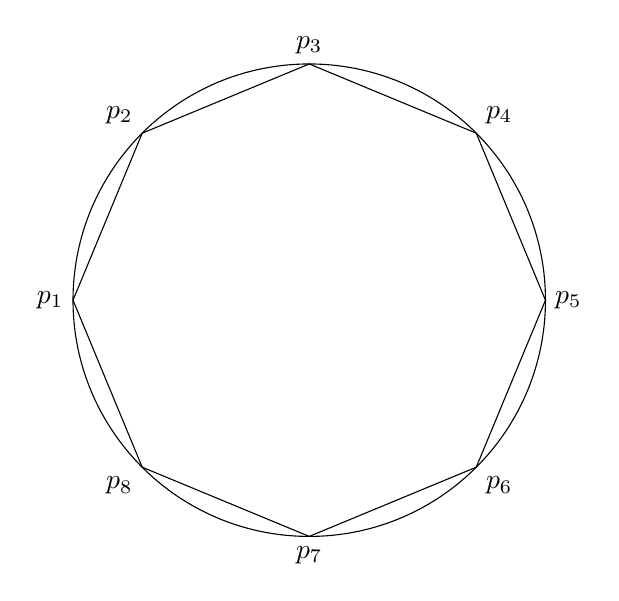
\begin{tikzpicture}[scale=1.5]
    \draw (0, 0) circle (2);
    \draw (-2, 0) node[left] {$p_1$} --
          (-1.414, 1.414) node[above left] {$p_2$} --
          (0, 2) node[above] {$p_3$} --
          (1.414, 1.414) node[above right] {$p_4$} --
          (2, 0) node[right] {$p_5$} --
          (1.414, -1.414) node[below right] {$p_6$} --
          (0, -2) node[below] {$p_7$} --
          (-1.414, -1.414) node[below left] {$p_8$} --
          (-2, 0);
  \end{tikzpicture}%
  \caption{Points $p_1, \cdots, p_8$ can be found by minimum / maximum x-coordinates, y-coordinates, differences / sums of x and y coordinates.
  Points within this octagon are not in the convex hull.}%
  \label{fig:akl}%
\end{figure}

A more recent example of point filtering can be found in ConcurrentHull~\cite{masnadi2020concurrent}, which effectively parallelizes a combination of Chan's algorithm~\cite{chan1996optimal} with convex hull point filtering.
They spatially partition the points on a grid, and remove the points of cells that are enclosed by other non\-/empty cells.
On a square point distribution, where the vast majority of points can be discarded in this manner, the approach achieves a speedup of up to \qty{40}{\times} over sequential Qhull.
It would be interesting to evaluate its performance on a circle, where significantly fewer points can be filtered out.
However, the implementation is restricted to integer coordinates, preventing a direct comparison.

It is also possible to do this preprocessing on the GPU~\cite{mei2016cuda}, to take advantage of its higher bandwidth compared to CPUs.
Do note that the bandwidth between GPU and system memory is typically lower than the bandwidth between CPU and system memory.
More closely related to this work is a GPU implementation of Eddy's algorithm~\cite{eddy1977convex}, a non\-/recursive version of Quickhull published 16 years earlier.
The absence of recursion makes it easier to implement on a GPU, but cannot take advantage of temporal locality and comes at a significant bookkeeping cost.

The sequential subset extraction is a straightforward adaptation of the vectorized partition algorithm used in QuickSort~\cite{bramas2017novel}.

\section{Future work}
This work implements planar Quickhull close to optimally on CPUs.
Nonetheless, we identify three directions of future work in relation to this algorithm.

First, it would be interesting to know if the practical performance of 3D Quickhull can be similarly improved.
A 3D convex hull cannot be straightforwardly represented as a flat array.
The main research question is what data structures are amenable to minimize data movement.
Our parallel extraction algorithm is tightly linked to a flat array, so this will not transfer directly.
The SIMD idea, however, can be used in higher dimensions as well.

Second, point filtering could further enhance the Quickhull algorithm.
We think a promising direction would be to implement Akl's heuristic using a modification of ips4o~\cite{axtmann2017inplace} in the same vein that our sequential extraction modifies Bramas' algorithm~\cite{bramas2017novel}.

Finally, future work should also explore whether this algorithm is suitable for GPUs.
We have already completed part of this work (which ended up being published earlier~\cite{koopman2025partitioning}) by porting the subset extraction for the special case $P = S_1 \sqcup S_2$.
This also provides worst\-/case and probabilistic bounds on the amount of data movement that the cleanup step has to do.
For a full GPU port, we still need to extend this to general subsets (relatively easy), and parallelize the recursion (more challenging).

More broadly, our observations suggest that dynamic software control can be an effective tool for balancing runtime and energy.
The runtime\-/optimal and energy\-/optimal configurations may not align, and the gap can vary across platforms, implementations, and datasets.
Determining these optima manually requires repeated benchmarking and platform\-/specific analysis.
Future systems could therefore adapt thread counts and other tuning parameters during execution time, rather than relying on a single static setting.

\section{Conclusion}
We present VQhull, a parallel algorithm for Quickhull.
Our implementation achieves an improvement of up to \qty{16}{\times} over the state\-/of\-/the\-/art sequential implementation.
By focusing on the memory subsystem rather than only on computational parallelism, the multithreaded implementation also improves on the state\-/of\-/the\-/art by up to \qty{11}{\times}.

Our implementation achieves \qtyrange{66}{100}{\percent} of the architecture's peak bandwidth, which suggests that the remaining headroom is \qtyrange{0}{50}{\percent}.
VQhull does best on systems with a single CPU and an instruction set that supports a compression instruction.
A system with multiple CPUs and a non\-/uniform memory architecture shows significant performance degradation for nested OpenMP parallelism, providing an opportunity for future work.

This algorithm also serves as a case study on engineering algorithms for energy efficiency.
We show that parallelizing programs can benefit energy efficiency by reducing clock frequency.
Energy savings on specific architectures are mostly in line with runtime improvements, but even when runtime savings are minimal, a well\-/thought\-/out implementation can still result in significant energy savings.
